\documentclass[prd,preprintnumbers,twocolumn,eqsecnum,floatfix,letter]{revtex4}
\usepackage{color}
\usepackage{calc}
\usepackage{amsmath,amssymb,graphicx}
\usepackage{amssymb,amsmath}
\usepackage{tensor}
\usepackage{bm}
\usepackage{times}
\usepackage[varg]{txfonts}
\usepackage[colorlinks, pdfborder={0 0 0}]{hyperref}
\definecolor{LinkColor}{rgb}{0.75, 0, 0}
\definecolor{CiteColor}{rgb}{0, 0.5, 0.5}
\definecolor{UrlColor}{rgb}{0, 0, 0.75}
\hypersetup{linkcolor=LinkColor}
\hypersetup{citecolor=CiteColor}
\hypersetup{urlcolor=UrlColor}
\maxdeadcycles=1000
\allowdisplaybreaks
\textwidth 7.5 in 
\hoffset -1 cm 
\newcommand{\RomanNumeralCaps}[1]{\MakeUppercase{\romannumeral #1}}
\newcommand{\comment}[1]{\textcolor{blue}{\textit{#1}}}
\newcommand{\ashok}[1]{\textcolor{red}{\textit{Ashok:#1}}}
\newcommand{\sean}[1]{\textcolor{cyan}{\textit{Sean:#1}}}


\begin{document}

\newcommand{\be}{\begin{equation}}
\newcommand{\ee}{\end{equation}}
\newcommand{\ber}{\begin{eqnarray}}
\newcommand{\eer}{\end{eqnarray}}
\def\bea{\begin{eqnarray}}
\def\eea{\end{eqnarray}}
\newcommand{\etal}{\emph{et al.}}

\newcommand{\Sl}{S_\ell}
\newcommand{\Sigmal}{\Sigma_\ell}
\newcommand{\Flux}{\mathcal{F}}
\newcommand{\LNh}{\hat{\mathbf{L}}_N}
\newcommand{\LN}{\mathbf{L}_N}
\newcommand{\bS}{\mathbf{S}}
\newcommand{\bJ}{\mathbf{J}}
\newcommand{\e}{\mathrm{e}}
\newcommand{\rmi}{\mathrm{i}}
\newcommand{\flow}{f_\mathrm{low}}
\newcommand{\fcut}{f_\mathrm{cut}}

\newcommand{\bchi}{\bm{\chi}}
\newcommand{\blambda}{\bm{\lambda}}
\newcommand{\bLambda}{\bm{\Lambda}}
\newcommand{\bchia}{\bm{\chi}_a}
\newcommand{\bchis}{\bm{\chi}_s}
\newcommand{\chis}{\chi_s}
%\newcommand{\bchi}{\mathbf{\chi}}
\newcommand{\chia}{\chi_a}
\newcommand{\chiadL}{\bchia \cdot \LNh}
\newcommand{\chisdL}{\bchis \cdot \LNh}
\newcommand{\chisSqr}{\bchis^2}
\newcommand{\chiaSqr}{\bchia^2}
\newcommand{\chisDchia}{\bchis \cdot \bchia}
\newcommand{\cA}{\mathcal{A}}
\newcommand{\cB}{\mathcal{B}}
\newcommand{\cC}{\mathcal{C}}
\newcommand{\cP}{\mathcal{P}}
\newcommand{\pc}{{+,\times}}

\title{Effect of Black Hole Spin on Christodoulou Memory}
\author{Ashok Choudhary}\email{aschoudhary@mix.wvu.edu}
\author{Sean T. McWilliams}\email{sean.mcwilliams@mail.wvu.edu}
\affiliation{Department of Physics and Astronomy, West Virginia University, Morgantown, WV 26506, USA}


\begin{abstract}
	The Christodoulou memory, which is a nonlinear memory effect sourced by the gravitational wave stress tensor, produce a growing, nonoscillatory change in the gravitational wave "plus" polarization. This results in the permanent displacement of a pair of freely falling test masses after the gravitational wave has passed. While the memory contribution during early in-spiral is well described by Post-Newtonian approximation, the contribution at merger must be obtained from Numerical relativity simulations. The Post-Newtonian corrections upto 3PN order to the gravitational wave memory for quasicircular, inspiralling compact binaries for non spinning has been computed by Favata et al.[Physical Review D 80, 024002 (2009)]. Here we include the Spin contribution at leading order and calculate the memory effect upto 3PN order. We also compute memory contribution at merger from Numerical relativity using Weyl curvature component $\psi_4$ after removing the unphysical low frequency contribution due to spectral leakage. We use the method described in [Class. Quantum Grav. 28 195015] for integration which control the amplification of the unphysical frequency resulting from spectral leakage. 
\end{abstract}

\maketitle

\section{Introduction}

Gravitational waves(GW), when they pass through a pair of freeling falling test masses cause an oscillatory motion. This oscillatory motion after the gravitational wave has passed through it, does not bring back the pair of test particle to their original location. This permanent displacement is called gravitational wave memory effect. This displacement is caused by a permanent deformation of spacetime geometry caused by passing gravitational waves. The memory effect associated with gravitational waves is accumulated effect over the entire lifehistory of the source. The permanent deformation that it leaves in spacetime geometry can be described in two ways: The Linear memory, which is caused by net change in the time derivative of source of one more multipole moment and the Nonlinear memory, which is caused by radiatiated gravitational waves acting as source for generating secondary gravitational waves. The linear memory is important for unbound astrophysical system and have been studied in context of supernova explosion, asymmetric mass loss due to neutrino emission, gamma-ray-burst jets etc \cite{Davies_Melvyn2002,Buonanno_Sigl2015,Kotake_Kei2009}. At leading order in a Post-Newtonian (PN) expansion, the linear memory causes a net change in the GW field given by
\begin{equation}
\Delta h^{TT}_{jk} = \frac{2}{R}\Delta\left(\ddot{\mathit{I}}^{TT}_{jk}\right) 
\end{equation} 
where $I_{ij}$ is the source mass-quadrupole moment, R is the distance to the source and $\Delta$ describes the net change in the quantity from early to late times. 
\par A general formula for the linear memory produced by an unbound system of N particle as a result of  change in  it’s mass $M_A$ and velocity configuration $v_A$ is given by Thorn \cite{Thorne_Braginskii1987} as shown below.
\begin{equation}\label{eq:1.2}
\Delta h^{TT}_{jk} = \Delta \sum_{A=1}^{N}\frac{4 M_A}{R\sqrt{1-v^2_A}}\left[\frac{v^j_A v^k_A}{1-\boldsymbol{v}_A\cdot \boldsymbol{N}}\right]
\end{equation} 

 Here $\Delta$ refers to take difference between the final and initial values of the summations, and $\boldsymbol{N}$ is the unit vector that points from the source to the observer.  
\\
The other kind of memory is the nonlinear memory, which is also called Christodoulou memory. It arises as results of change in the radiative multipole moment that is sourced by the energy flux of the radiated GWs. It can be understood by looking at Eisntein's equations in harmonic gauge and considering the leading order nonlinear terms. The equation below shows a wave equation for spacetime metric in harmonic gauge with different source terms appearing on the right. \cite{Thorne1980} 
\begin{subequations}
\begin{align}\label{eq:3.1a}	
\Box \bar{h}^{\alpha \beta} & = -16\pi (-g)(T^{\alpha\beta} + t_{LL}^{\alpha\beta})-\bar{h}^{\alpha\mu}_{,\nu}\bar{h}^{\beta\nu}_{,\mu}+\bar{h}^{\mu\nu}\bar{h}^{\alpha\beta}_{,\mu\nu}\\
\bar{h}^{\alpha \beta},_{\beta} & = 0
\end{align}
\end{subequations}
where
\begin{equation}
\bar{h}^{\alpha \beta} = \eta^{\alpha\beta}-\sqrt{-g}g^{\alpha\beta} 
\end{equation}
is the gravitational field tensor, $g$ is the determinant of the metric $g_{\alpha\beta}$, $T^{\alpha\beta}$ is the matter stress-energy tensor, $t^{\alpha\beta}_{LL}$ is the Landau-Lifshitz pseudotensor, $\Box \equiv  -\partial^{2}_{t} + \nabla^{2}$ is the flat-space wave operator, a comma denotes a partial derivative $(,_{\mu}\equiv \partial_{\mu})$, and $\nabla^{2}$ is a flat-space Laplace operator. We can see that there are many source terms.The Landau-Lifshitz term is the Gravitational wave stress tensor which is the source of nonlinear memory contribution to GW waveform.~\cite{Isaacson1968}.
\begin{equation}
	T^{gw}_{jk}=\frac{1}{32\pi}\langle h^{TT}_{ab,j}h^{TT}_{ab,k}\rangle\approx T^{gw}_{00}n_{j}n_{k} = \frac{1}{R^{2}}\frac{dE^{gw}}{dt d\Omega}n_{j}n_{k}
\end{equation}
where $\frac{dE^{gw}}{dtd\Omega}$ is the GW energy flux, $n_{j}$ is a unit radial vector, the angle-bracket mean to average over several wavelengths, $h^{TT}_{ab}=\bar{h}^{TT}_{ab}$. The standard procedure to solve a wave equation with source is by using Green’s function. When applied to  Eq. \ref{eq:3.1a} obtains a correction term to gravitational field sourced by the Landau-Lifshitz term is shown below \cite{Wiseman1991}
\begin{equation}\label{eq:1.6}
	\delta h^{TT}_{jk} = \frac{4}{R}\int_{-\infty}^{T_{R}} dt'\Bigg[ \frac{dE^{gw}}{dt'd\Omega'}\frac{n'_{j}n'_{k}}{(1-\boldsymbol{n'}\cdot\boldsymbol{N})}d\Omega'\Bigg]^{TT}
\end{equation}
where $T_{R}$ is the retarded time. The above equation \ref{eq:1.6} gives the nonlinear Landau-Lifshitz pseudotensor term contribution to gravitational wave memory. This was independently discovered by Christodoulou \cite{Christodoulou1991}, Payne \cite{Payne1894}, Blanchet and Damour \cite{Blanchet_Damour1992}. The nonlinear memory occurs in any system that radiates GWs. These systems are usually considered to have a vanishing linear memory. The nonlinear memory [Eq.\ref{eq:1.6}] can be described by equation \ref{eq:1.2}, the formula for the linear memory if the unbound object in the system are taken to be the individual gravitons with energy $E_A = M_A/(1-v_A^2)^{1/2}$ and velocities $v_A^j = c\,{n'}_A^{j}$.\cite{Thorne1992} 
\par The Christodoulou memory effect arises from nonlinear interactions at 2.5 PN order but affects the gravitational waveform at leading (0PN) order. The $+$ polarization of the gravitational wave signal starts to ossillates around zero and slowly starts to deviate dues to Chritodoulou memory effect. This oscillatory shift in the amplitude of $+$ polarization starts at early times and slowly grows during inspiral phase. The PN waveform allow us to model the slow growth of memory during the inspiral phase of coalescence, but the most contribution to this nonlinear memory come from the merger phase where the PN model do not work. In this case the memory must be extracted from Numerical relativity (NR) simulations. However, it is quite challenging to extract the nonlinear memory accurately from numerical simulations of binary black holes. NR simulations can most accurately compute the $(l, m) = (2, 2)$ mode of the waveform; but the nonlinear memory is present in only $m=0$ mode. These $m=0$ modes are much smaller in magnitude and depends more sensitively on	initial conditions than other modes. For detailed discussion on this see section $\RomanNumeralCaps{5}$ in reference \cite{Favata2009}
\par The NR simulations mostly easily compute  the curvature scalar $\Psi_4$ and decompose its values at large $R$ into a sum over spin-weighted spherical harmonic modes:
\begin{equation}
	\Psi_4 = \ddot{h}_+ - \mathit{i}\ddot{h}_\times = \sum_{l=2}^{\infty}\sum_{m=-l}^{l}\psi_{lm}(t, R) _{-2}Y_{lm}(\Theta, \Phi)
\end{equation} 
In terms of the $\psi_{lm}$ modes, the leading-order Christodoulou-memory modes are smaller than the $\psi_{22}$ modes by $five$ PN orders. The relative mode magnitudes(\cite{Favata2009}) are $\psi_{22} \approx 690 \psi_{20}\approx 4.5 \times 10^4 \psi_{40}$ at $x\approx1/5$. There are other difficulties too in calculating memory from numerical relativity data. Construction of the $h_{lm}$ from $\psi_{lm}$ requires two integration constants to be specified. Choosing these integration constant to be zero \cite{Reisswig_Pollney2011}  does not make the signal oscillate around zero. Although it should not if memory is present, but this nonlinear growth is not solely due to actual memory effect. This can also be caused by numerical noise. So there is an artificial memory in the $h_{lm}$ modes which is caused by numerical noise. This artificial memory is unphysical and arises from the finite size of the initial separation and extraction radius. The initial burst of junk radiation also contribute to artificial memory.
\par Numerical relativity simulations starts at a finite radius, so although it contains most part of gravitational wave memory, PN results should be used for early inspiral phase. The significance of memory accumulated during the inspiral phase can be seen by looking at the largest memory mode $h_{20}$. Consider the leading-(Newtonian)-order piece of the largest memory mode $h_{20}$:
\begin{equation}
	h^{NR}_{20}\left(T_R\right) = \frac{1}{\sqrt{2}R}\int_{T_0}^{T_R}U^{(mem)(1)}_{20}(t)dt
\end{equation}
where $U^{(mem)(1)}_{20}$ is given by the leading order piece of Eq. (3.13a) in ref \cite{Favata2009}, and the $T_0$ is the starting time of the simulation. For a realistic, quasicircular binary that inspirals from a large initial separation, $T_0 \rightarrow -\infty$. The NR simulations of binaries that starts at a finite initial separation would underestimate the size of the memory. For a simulation that starts with an initial separation of $10M$, the error in the memory at a harmonic coordinate separation of $5M$ is $50\%$.\cite{Favata2009} 

\par The corrections to the leading-oder formula for the nonlinear memory's contribution to 3PN order for non-spinning binaries has been computed by by Favata \cite{Favata2009}. However the effect of binary spins have not been explored in these results. Astrophysical black holes are formed by gravitation collapse of massive star when when they run out of their nuclear fuel in the core. These massive stars are likely to posses spin angular momentum, as a result the black hole formed would also be spinning. The black holes can also accrete matter from surrounding and as a result spin up during the process. It is highly likely that there is a large population of spinning binaries in the universe.      
\par In this paper we calculate the nonlinear memory contribution to the + waveform polarization and look at the effect of spin contribution. For PN calculations, this paper is just an extension of Favata's\cite{Favata2009} paper, where we include the spin contribution upto leading (1.5 PN) order for nonprecessing binaries. The nonlinear memory contribution near merger is computed using NR data from publicly available SXS catalog, where we process the data to remove the low frequency numerical noise. In Sec. II, we describe the calculation required to compute memory contribution to the post-Newtonian waveform of quasi-circular, inspiralling binaries. In Sec. III, we describe the method used to extract memory contribution from NR simulations. Sec. IV we give the results which looks at the effect of spin on total nonlinear memory. We use PN expressions for memory for early time and for late time we use memory extracted from NR simulations.


\section{MEMORY CONTRIBUTION TO POST-NEWTONIAN WAVEFORM POLARIZATION}

The mode decomposition in terms spin-weighted spherical harmonics for gravitational wave polarization is given by
\begin{equation}\label{eq:2.1}
	h_+ - \mathit{i}h_{\times} = \sum_{l=2}^{\infty}\sum_{m=-l}^{m=l}h^{lm} \,  _{-2}Y^{lm}(\Theta, \Phi)
\end{equation}
where $_{-2}Y^{lm}$ are spin-weighted spherical harmonics, the angles $(\Theta, \Phi)$ indicates the direction from the source to the observer. In a multipolar expansion of the GW field, the modes $h^{lm}$ are related to the radiative mass $U^{lm}$ and the current $V^{lm}$ multipole via
\begin{equation}\label{eq:2.2}
	h^{lm}= \frac{G}{\sqrt{2}\, R }\left[U^{lm}(T_R)-\frac{\mathit{i}}{c}V^{lm}(T_R)\right]
\end{equation}
Here $R$ is the distance from source to observer, $T_R$ is retarded time. We assume $c\,=\,G\,=\,1$ for all out calculations.
 The spin weighted spherical harmonics are defined in terms of the Wigner $d$ function by
\begin{equation}\label{eq:2.3}
	_{-2}Y^{lm}(\Theta, \Phi) = (-1)^2\sqrt{\frac{2l + 1}{4\pi}}d^{l}_{ms}(\Theta)e^{\mathit{i}m\Phi}
\end{equation} 
Here
\begin{align}\label{eq:2.4}
	d^{l}_{ms}&=\sqrt{(l+m)!(l-m)!(l+s)!(l-s)!}\\
	&\times \sum_{k=k_i}^{k_f}\frac{(-1)^k(\sin\frac{\Theta}{2})^{2k+s-1}(\cos\frac{\Theta}{2})^{1l+m-s-2k}}{k!(l+m-k)!(l-s-k)!(s-m+k)!}
\end{align}
where $k_i$ = max$(0, m-s)$ and $k_f$ = min$(l+m, l-s)$. \\
When the GW field is decomposed into spin-weighted spherical harmonic modes, the nonlinear memory can be shown to yield a correction to the radiative mass multipole moments that enters at 2.5PN and higher orders. For more detail about GW multipole expansion \cite{Thorne1980}. The correction to the radiative mass multipole moments is given by
\begin{equation}\label{eq:2.6}
	U^{(mem)}_{lm}=32\pi\frac{(l-2)!}{2(l+2)!}\int_{-\infty}^{T_R}dt\int d\Omega\frac{dE_{gw}}{dtd\Omega}(\Omega)Y^*_{lm}(\Omega)
\end{equation}
The radiative current moments $V_{lm}$ do not contribute to nonlinear memory. The GW energy flux can be computed from the GW stress-energy tensor and is given by \cite{Favata2010}
\begin{equation}\label{eq:2.7}
	\frac{dE_{gw}}{dtd\Omega} = R^2 T^{gw}_{00} = \frac{R^2}{32\pi}\langle\dot{h}^{TT}_{jk}\dot{h}^{TT}_{jk}\rangle =\frac{R^2}{16\pi}\langle\dot{h}^2_{+}+ \dot{h}^2_{\times}\rangle
\end{equation}
where the angled bracket mean to average over several wavelengths. The energy flux can be written in terms of $h_{lm}$ modes using equation \ref{eq:2.1} in the following way:
\begin{widetext}
\begin{equation}\label{eq:2.8}
		\frac{dE_{gw}}{dtd\Omega}=\frac{R^2}{16\pi}\sum_{l'=2}^{\infty}\sum_{l''=2}^{\infty}\sum_{m'=-l'}^{l'}\sum_{m''=-l''}^{l''}\langle\dot{h}_{l'm'}\dot{h}^*_{l''m''}\rangle _{-2}Y^{l'm'}(\theta,\phi)_{-2}Y^{l''m''*}(\theta, \phi)
\end{equation}
\end{widetext}

The memory contribution to the mass multipole moment can now be evaluated using equation \ref{eq:2.6} and \ref{eq:2.8}. The angular part of the integral has the following form

\begin{equation}\label{eq:2.9}
	\int d\Omega _{-2}Y_{l'm'}(\theta,\phi)_{-2}Y_{l''m''}^{*}(\theta, \phi)Y_{lm}^{*}(\theta, \phi)
\end{equation}

The above integral can be evaluated as done in section III of  Favata\cite{Favata2009}. The results are also shown in appendix ~\ref{Appendix A}. The time derivative of the memory mass-multipole moment is defines as $U^{(mem)(1)}_{lm}\equiv\frac{dU^{(mem)}_{lm}}{dT_R}$ \cite{Favata2009}, which when combined using equation \ref{eq:2.6} and \ref{eq:2.8} and Appendix \ref{Appendix A}, can be written as

\begin{align}\label{eq:2.10}
	U_{lm}^{(mem)(1)}=&R^{2}\sqrt{\frac{2(l-2)!}{(l+2)!}}\sum_{l'=2}^{\infty}\sum_{l''=2}^{\infty}\sum_{m'=-l'}^{l'}\sum_{m''=-l''}^{l''}(-1)^{m+m'}\nonumber\\
	&\times\Bigg\langle \dot{h}_{l'm'}\dot{h}_{l'm'}^{*}\Bigg\rangle G^{2-20}_{l'm'lm'-m''-m}
\end{align}
 
where $G^{2-20}_{l'm'lm'-m''-m}$ is the angular integral of equation \ref{eq:2.9} and is given in Appendix \ref{Appendix A}. The above equation can be used to compute the first time derivative of mass-multipole moment by substituting the GW modes $h_{lm}$. When evaluating equation \ref{eq:2.10}, we are only interested in $m=0$ modes. The $m\neq0$ terms yield oscillatory contribution to the waveform polarizations that enter at higher PN orders then the nonoscillatory, $m=0$ terms. The non-vanishing, non-oscillatory modes are $U^{(mem)}_{l0}$ with l-even. These $U^{(mem)}_{l0}$ consist of time-integral of polynomials in $x\equiv(M\omega)^{2/3}$ (where $\omega$ is the orbital angular frequency), with each terms of the form
\begin{equation}\label{eq:2.11}
\int_{-\infty}^{T_{R}} x^{n}dt=\int_{-\infty}^{T_{R}}\frac{x^{n}}{\dot{x}}dx
\end{equation}
After performing the change of variable indicated in above equation \ref{eq:2.11}, evaluation of the resulting integrals requires a model for the frequency evolution of the binary. The adiabatic evolution of the frequency (or $x$) is easily derived from energy balance ($\mathcal{L}_{GW}=-\dot{E}$). and the relation $\dot{x}=-\mathcal{L}_{GW}/(dE/dx)$. The 3.5PN orbital energy and flux are given in Appendix C of reference \cite{Arun2009}. Here we who only upto 1.5 PN terms, the complete expression are show in Appendix \ref{Appendix:C1}. The 1.5 PN expression for energy is given by 
\begin{widetext}
	\begin{align}\label{eq:E}
	E&=-\frac{\eta \, M \, x}{2}\left\{1 + x \left[-\frac{3}{4}-\frac{\eta}{12}\right] + x^{3/2}\left[\left(\frac{8}{3} - \frac{4 \, \eta}{3}\right)\chisdL + \frac{8}{3}\delta\chiadL\right]\right\} \nonumber \\
	\end{align}

and the 1.5 PN GW luminosity is given by

\begin{align}\label{eq:F}
\mathcal{L} &=\frac{32}{5}\eta^2x^5\left\{1 + x\left[-\frac{1247}{336}-\frac{35\,\eta}{12}\right] + x^{3/2}\left[4\pi-\left\{\left(\frac{11}{4}-3\eta\right)\chisdL +\frac{11}{4}\delta\chiadL\right\}\right]\right\}\nonumber\\
\end{align}


Substituting the above two equation into $\dot{x}=-\mathcal{L}_{GW}/(dE/dx)$, and expanding upto 1.5 PN gives the following expression.

\begin{align}\label{eq:2.14}
\frac{dx}{dt} & = \frac{64\, x^5  \, \eta}{5} \left\{1 + x \left[-\frac{743}{336}-\frac{11 \eta }{4} \right] 
+ x^{3/2} \left[4 \pi-\frac{113}{12}\delta \, \chiadL- \left(-\frac{113}{19} + \frac{19 \, \eta}{3}  \right)\chisdL \right] \right\} \nonumber \\ 
\end{align}
\end{widetext}
The results upto 3.5 PN are shows in Appendix \ref{Appendix:C}.
The equation \ref{eq:2.14} can be used to change the integration with respect to time into integration with respect to $x$ as shown in equation in \ref{eq:2.11}. The expressions for $h_{lm}$ whose first time derivatives appear equation \ref{eq:2.10} can be obtained from Ref\cite{Arun2009}. The GW modes for precessing binaries with small inclination angle on nearly circular orbits through 1.5 PN order are given in section IV of ref \cite{Arun2009}. Setting $\iota = 0, \alpha = \pi$ in equation 4.16 and 4.17 gives the result for non-precessing case. In that case the spins are aligned along $z$ axis, so we set $\chi_a^x=\chi_s^x=\chi_a^y=\chi_s^y=0$. We can now write the expression as 
\begin{equation}
h_{lm} = (-1)^{m+1}\frac{(2M\eta v^2)}{D_L}\sqrt{\frac{16\pi}{5}}e^{\mathit{i}\,m\,\psi}\hat{h}_{lm},
\end{equation}
and $\hat{h}_{lm}$ modes are given by 
\begin{subequations}
	\begin{align}\label{eq:2.15}
	\hat{h}_{22} &= 1 + x\left(-\frac{107}{42} + \frac{55\eta}{42}\right) + x^{3/2}\left(2\pi - \frac{4\,\delta\,\chi^{z}_{a}}{3} + \frac{4}{3}\left(-1+\eta\right)\chi^z_s\right)\\
	\hat{h}_{21} &= \frac{\mathit{i}\delta}{3}\left[x^{1/2} - x\frac{3}{2\delta}\left(\chi^{z}_{a} + \delta\chi^{z}_{s}\right) + x^{3/2}\left(-\frac{17}{28} + \frac{5\eta}{7}\right)\right]\\
	\hat{h}_{32} &= \frac{9}{8}\sqrt{\frac{5}{7}}\left[\frac{8}{27}x\left(1-3\nu\right) + \frac{32}{27}x^{3/2}\eta\,\chi^z_s\right]
	\end{align}
\end{subequations}
The remaining $h_{lm}$ expressions does not contain spin terms and the complete expressions upto 3PN terms can be directly taken from Ref.\cite{Blanchet_Iyer2008}
 We show the $h_{lm}$ expressions for positive $m$ values, but the results for negative $m$ values can be obtained by the relation, $h_{l, -m} = (-1)^l \bar{h}_{lm}$. This results is not in general true for precessing binaries, but it continues to hold true of non-precessing case. The time derivative of $h_{lm}$ modes can be obtained by following the procedure shown in Appendix \ref{Appendix B}. With these modes we use equation \ref{eq:2.10} to evaluate the first time derivative of the memory mass-multipole moment, which is further integrated using equation \ref{eq:2.11}. The results after integration are show in next section.

\begin{widetext}
\subsection{RESULTS: MEMORY CONTRIBUTION TO THE POST-NEWTONIAN WAVEFORM OF QUASI-CIRCULAR, INSPIRALLING BINARIES}
The memory contribution to the spin-weighted spherical-harmonic modes of the polarization waveform [Eq. \ref{eq:2.2}]. These quantities are related via 
\begin{equation}
	h_{l0}^{(mem)} = \frac{\alpha}{\sqrt{2} \, R} U_{l0}^{(mem)} = 8 \sqrt{\frac{\pi}{5}}\frac{\eta M x}{R}\hat{H}_{lm}
\end{equation}
where we have followed the notation of Sec. 9 of Ref. \cite{Blanchet_Iyer2008}. The parameter $\alpha$ takes the value as shown below, depending upon the polarization triad chosen. 
\begin{equation}
\alpha = \left\{
\begin{array}{ll}
(+1) & \text{for the Kidder  \cite{Kidder2008} convention} \\
(-1) & \text{for the Blanchet et al. \cite{Blanchet_Iyer2008}   convention}\\
\end{array} 
\right.
\end{equation}

The results of polarization modes in terms of $\hat{H}_{l0}$ are:
\begin{subequations}
\begin{align}\label{eq:H20}
&\hat{H}_{20} = \alpha \frac{5}{14\sqrt{6}}\left\{ 1 + x\left[-\frac{4075}{4032} + \frac{67 \, \eta}{48}\right]+ x^{3/2}\left[\left(\frac{7}{480} +\frac{27 \, \delta}{10} - \frac{7 \,\eta}{120}\right)\chiadL+\left(\frac{27}{10} +\frac{7 \, \delta^3}{480} - \frac{2 \, \eta}{15}\right)\chisdL\right]\right. \nonumber \\
& \quad \left. x^2\left[-\frac{151877213}{67060224} -\frac{123815 \, \eta}{44352} +\frac{205 \, \eta^2}{352} +\left(-\frac{163}{96} +\frac{161 \, \eta}{24}\right)\chiaSqr + \left(-\frac{27 \, \delta}{8} -\frac{\delta^3}{48}\right)\chisDchia + \left(-\frac{27}{16}-\frac{\delta^4}{96} -\frac{\eta}{12}\right)\chisSqr\right]\right. \nonumber \\
& \quad \left. x^{5/2}\left[-\frac{253 \, \pi}{336}+ \frac{253 \, \pi \, \eta}{84} +\left\{\frac{631}{32256} + \frac{788471\,\delta}{84672} +\left(-\frac{5}{126}-\frac{991\,\delta}{1008}\right)\eta-\frac{311\,\eta^2}{2016}\right\}\chiadL\right.\right. \nonumber\\
& \qquad\left. +\left\{\frac{788471}{84672}-\frac{631\, \delta^3}{32256} -\left(-\frac{36509}{2646} + \frac{311\,\delta^3}{8064}\right)\eta+\frac{853\,\eta^2}{252}\right\}\chisdL\right] \nonumber \\
& \quad  x^3\left[-\frac{4397711103307}{532580106240} + \left( \frac{700464542023}{13948526592} - \frac{205 \, \pi^2}{96}\right)\eta + \frac{69527951 \, \eta^2}{166053888} + \frac{1321981 \, \eta^3}{5930496} -  \left(-\frac{7\,\pi}{256} + \frac{275\,\pi\,\delta}{12} \right.\right. \nonumber \\
& \qquad \left. \frac{7 \, \pi\,\delta}{256}\right)\chiadL + \left\{-\frac{42787}{32256} + \frac{791\,\delta}{9216} +\frac{113\,\delta^2}{576} + \left(\frac{354035}{32256} -\frac{791\,\delta}{2304}\right)\eta - \frac{2533\,\eta^2}{128}\right\}\chiaSqr\nonumber\\
&\qquad \left.\left. \left\{\frac{275\,\pi}{12} -\frac{7\,\pi\,\delta^3}{256}-\frac{56\,\pi\eta}{3} + \left(\frac{791}{9216} -\frac{47869\,\delta}{21504}-\frac{743\,\delta^3}{21504} + \frac{791\,\delta^4}{9216} + \left(-\frac{77}{192}+\frac{87269\, \delta}{2304}-\frac{11\, \delta^3}{256}\right)\eta + \frac{133\,\eta^2}{576}\right)\chiadL\right\}\chisdL\right.\right.\nonumber\\
& \qquad \left.\left.\left\{-\frac{47869}{43008} + \frac{791\,\delta^3}{9216} -\frac{743\,\delta^4}{43008} + \left(\frac{57677}{1792} -\frac{133\,\delta^3}{2304} -\frac{11\,\delta^4}{512}\right)\eta - \frac{15029\,\eta^2}{1152}\right\}\chisSqr
\right]\right\}
\end{align}


\begin{align}\label{eq:H40}
	&\hat{H}_{40} =\alpha\frac{1}{504\sqrt{2}}\left\{1 + x\left[-\frac{180101}{29568} + \frac{27227\,\eta}{1056}\right] + x^{3/2}\left[\left(\frac{7}{40} + \frac{27\,\delta}{10} -\frac{7\,\eta}{10}\right)\chiadL+\left(\frac{27}{10}+\frac{7\,\delta^3}{40} +\frac{46\,\eta}{5}\right)\chisdL\right]\right.\nonumber\\
	&\qquad x^{5/2}\left[-\frac{13565\,\pi}{1232} + \frac{13565\,\pi\,\eta}{308} + \left\{\frac{379}{2688}-\frac{1457321\,\delta}{68992}+\left(-\frac{59}{336} + \frac{3094367\,\delta}{22176}\right)\eta -\frac{87\,\eta^2}{56}\right\}\chiadL\right.\nonumber\\
	&\qquad\qquad \left. \left\{-\frac{1457321}{68992} + \frac{379\,\delta^3}{2688} + \left(\frac{5892749}{38808} + \frac{87\,\delta^3}{224}\eta-\frac{469813\,\eta^2}{5544}\right)\right\}\chisdL\right]\nonumber\\
	&\quad\qquad x^2\left[\frac{2201411267}{158505984} -\frac{34829479\,\eta}{432432} + \frac{844951\,\eta^2}{27456} + \left(-\frac{85}{48} + 7\,\eta\right)\chiaSqr + \left(-\frac{27\, \delta}{8} -\frac{\delta^3}{6}\right)\chisDchia + \left(-\frac{27}{16} -\frac{\delta^4}{12} + \frac{\eta}{12}\right)\chisSqr\right].\nonumber\\
	&\quad\qquad x^3\left[\frac{167644780815461}{8592292380672}+\left(-\frac{11327099812895}{306867585024} -\frac{205\,\pi^2}{96}\right)\eta -\frac{137763118975\,\eta^2}{1217728512} + \frac{2435519695\,\eta^3}{130470912}\right.\nonumber\\
	&\qquad\qquad  + \left(-\frac{21\,\pi}{64} + \frac{275\,\pi\,\delta}{12} + \frac{21\,\pi\,\eta}{16}\right)\chiadL + \left(\frac{32394371}{2838528} + \frac{791\,\delta}{768} + \frac{113\,\eta^2}{576} + \left(-\frac{71832779}{709632} -\frac{791\,\delta}{192}\right)\eta + \frac{59317\,\eta^2}{264}\right)\chiaSqr .\nonumber\\
	&\qquad\qquad + \left\{\frac{275\,\pi}{12} - \frac{21\,\pi\,\delta^3}{64} -\frac{91\,\pi\,\eta}{3} + \left(\frac{791}{768} + \frac{11114513\,\delta}{473088} -\frac{743\,\delta^3}{2688} + \frac{791\,\delta^4}{768} + \left(-\frac{77}{16} -\frac{649327\,\delta}{16896} -\frac{11\,\delta^3}{32}\right)\eta  \right.\right.\nonumber\\
	&\qquad\qquad \left.\left.\left. \left.+ \frac{133\,\eta^2}{48}\right)\chiadL\right\}\chisdL + \left(\frac{11114513}{946176} + \frac{791\,\delta^3}{768} -\frac{743\,\delta^4}{5376} + \left(\frac{2007451}{118272} -\frac{133\,\delta^3}{192} -\frac{11\,\delta^4}{64}\right)\eta - \frac{82411\,\eta^2}{2816}\right)\chisdL\right]\nonumber
	\right\}\\
\end{align}	

\begin{align}\label{eq:H60}
	&\hat{H}_{60} =-\alpha\frac{4195}{1419264\sqrt{273}}x\left\{1-\frac{3612\,\eta}{839}+ x\left[-\frac{45661561}{6342840} + \frac{101414\,\eta}{2517} - \frac{48118\,\eta^2}{839}\right]\right. + x^{3/2} \left[\frac{1248\,\pi}{839} -\frac{4992\,\pi\,\eta}{839}\right.\nonumber\\
	&\qquad + \left(-\frac{44}{5873} + \frac{14129\,\delta}{2517} + \left(\frac{264}{5873} - \frac{140148\,\delta}{5873}\right)\eta -\frac{352\,\eta^2}{5873}\right)\chiadL + \left(\frac{14129}{2517} -\frac{44\,\delta^3}{5873}\right.\nonumber\\
	&\quad\qquad + \left.\left.\left(-\frac{79120}{2517} + \frac{88\,\delta^3}{5873}\right)\eta + \frac{161136\,\eta^2}{5873}\right)\chisdL\right] + x^{5/2}\left[\frac{66616409\,\pi}{2718360} -\frac{874693\,\pi\,\eta}{7551} + \frac{239134\,\pi\,\eta^2}{2517}\right. + \nonumber\\
	&\qquad\qquad \left(-\frac{8173}{634248} -\frac{1240441999\,\delta}{57085560} + \left(\frac{6479}{105714} + \frac{15116383\,\delta}{105714}\right)\eta + \left(-\frac{1100}{158571}-\frac{2406356\,\delta}{7551}\right)\eta^2-\frac{968\,\eta^3}{7551}\right)\chiadL\nonumber\\
	&\qquad\qquad \left. \left(-\frac{1240441999}{57085560} -\frac{8173\,\delta^3}{634284} + \left(\frac{2016684797}{14271390} + \frac{3091\,\delta^3}{317142}\right)\eta + \left(-\frac{19243010}{52857} + \frac{242\,\delta^3}{7551}\right)\eta^2 + \frac{1891144\,\eta^3}{7551}\right)\chisdL\right]\nonumber\\
	&\qquad x^2\left[\frac{33133408041593}{1594133291520}-\frac{912563795039\,\eta}{25102880} + \frac{8054229309\,\eta^2}{25102880}-\frac{1363643519\,\eta^3}{18827160} + \left(-\frac{81}{32} + \frac{140263\,\eta}{6712}-\frac{36120\,\eta^3}{839}\right)\chiaSqr\right. \nonumber\\
	& \quad\qquad \left.+ \left(-\frac{81\,\delta}{16} + \frac{73143\,\delta\,\eta}{3356}\right)\chisDchia + \left(-\frac{81}{32} + \frac{36991\,\eta}{3356} - \frac{7047\,\eta^2}{1678}\right)\chisSqr\right]
\end{align}

\begin{align}\label{eq:H80}
	&\hat{H}_{80} =\alpha\frac{75601}{213497856\sqrt{119}}x^2\left[1-\frac{452070\,\eta}{75601} + \frac{733320\,\eta^2}{75601} + x\left(-\frac{265354303}{33869248} + \frac{18177343651\,\eta}{321757856} - \frac{5057483259\,\eta^2}{40219732} + \frac{1828935981\,\eta^3}{20109866}\right)\right]\nonumber\\	
\end{align}
\begin{align}\label{eq:H80}
\hat{H}_{100} &=-\alpha\frac{525221\,x^3}{6452379648\sqrt{154}}\left(1 - \frac{79841784\,\eta}{9979199} + \frac{198570240\,\eta^2}{9979199} -\frac{172307520\,\eta^3}{9979199}\right)
\end{align}
\end{subequations}
We can see that all contribution to $m=0$, even-$l$ modes arise solely from the Christodoulou memory piece of $U_{lm}$. There are no hereditary-memory contribution to the radiative current multipole moments $V_{lm}$\\
We can combine the above with equation \ref{eq:2.1} and explicitly compute the memory contribution to the + waveform polarization.This can be done in the following way

\begin{equation}
	h_{+,\times} = \frac{2\eta Mx}{R}H_{+,\times} + O\left(\frac{1}{R^2}\right)
\end{equation}
\begin{equation}
	H_{+,\,\times}= \sum_{n=0}^{\infty}x^{n/2}H_{+,\,\times}^{(n/2)}
\end{equation}
The memory contribution to $H_{+}^{n/2} $ are:
\begin{subequations}
\begin{align}
	& H_{+}^{(0,mem)}=\alpha\frac{1}{96}s_{\Theta}^2\left(17 + c_{\Theta}^2\right),\\
	& H_{+}^{(0.5,mem)}=0,\\
	& H_{+}^{(1,mem)}=\alpha s_{\Theta}^2\left[-\frac{354241}{2064384} - \frac{62059}{1032192}c_{\Theta}^2 - \frac{4195}{688128}c_{\Theta}^4 + \eta\left(\frac{15607}{73728} + \frac{9373}{36864}c_{\Theta}^2 +\frac{215}{8192}c_{\Theta}^4\right)\right],\\
	& H_{+}^{(1.5,mem)}=\alpha s_{\Theta}^2\left\{\left[\frac{3}{1280}  + \frac{7}{3840}c_{\Theta}^2 +  \delta\left(\frac{153}{320} + \frac{9}{320}c_{\Theta}^2\right) +\eta \left(-\frac{3}{320}-\frac{7}{960}c_{\Theta}^2\right)\right]\chiadL\right.\nonumber\\
	& \qquad\qquad+\left.\left[\left(\frac{153}{320} + \frac{9}{320}c_{\Theta}^2\right) + \delta\left(\frac{3}{1280} + \frac{7}{3840}c_{\Theta}^2\right) + \eta\left(-\frac{3}{80} +\frac{23}{240}c_{\Theta}^2\right) + \delta\eta\left(-\frac{3}{320}-\frac{7}{960}\right)\right]\chisdL\right\}\nonumber\\
	\\
	& H_{+}^{(2,mem)} =\alpha s_{\Theta}^2\left\{-\frac{3968456539}{9364045824} + \frac{570408173}{4682022912}c_{\Theta}^2 + \frac{122166887}{3121348608}c_{\Theta}^4 + \frac{7560}{15925248}c_{\Theta}^6 \right.\nonumber\\
	& \qquad\qquad + \eta\left[-\frac{7169749}{18579456} - \frac{13220477}{18579456}c_{\Theta}^2 -\frac{1345405}{6193152}c_{\Theta}^4 - \frac{25115}{884736}c_{\Theta}^6\right] + \eta^2\left[\frac{10097}{147456} + \frac{5179}{36864}c_{\Theta}^2 + \frac{44765}{147456}c_{\Theta}^4\right.\nonumber\\
	& \qquad\qquad\quad \left.+ \frac{3395}{73728}c_{\Theta}^6\right] + \left[-\frac{1385}{4608}-\frac{85}{4608}c_{\Theta}^2 +\eta\left(\frac{19}{16} + \frac{7}{96}c_{\Theta}^2\right)\right]\chiaSqr + \left[-\frac{1385\sqrt{1-4\eta}}{2304} - \frac{85\sqrt{1-4\eta}}{2304}c_{\Theta}^2\right.\nonumber\\
	& \qquad\qquad\quad \left. \left.+ \eta\left(\frac{\sqrt{1-4\eta}}{72} + \frac{\sqrt{1-4\eta}}{144}c_{\Theta}^2\right)\right]\chisDchia + \left[-\frac{1385}{4608}-\frac{85}{4608}c_{\Theta}^2 + \eta^2\left(-\frac{1}{36}-\frac{c_{\Theta}^2}{72}\right)+ \eta\left(\frac{11}{384} + \frac{c_{\Theta}^2}{128}\right)\right]\chisSqr\right\}\nonumber\\
	\\
	& H_{+}^{(2.5,mem)} =\alpha s_{\Theta}^2\left\{-\frac{2545\pi}{21504} - \frac{295\pi}{2688}c_{\Theta}^2 -\frac{65\pi}{7168}c_{\Theta}^4 + \eta\left[\frac{2545\pi}{5376} + \frac{295\pi}{672}c_{\Theta}^2 + \frac{65\pi}{1792}c_{\Theta}^4\right] + \left[\frac{11867}{3612672} + \frac{8156279\sqrt{1-4\eta}}{4816896}\right.\right.\nonumber\\
	& \qquad\qquad\quad + \frac{163}{112896}c_{\Theta}^2 - \frac{484979\sqrt{1-4\eta}}{2408448}c_{\Theta}^2 + \frac{55}{1204224}c_{\Theta}^4 -\frac{70645\sqrt{1-4\eta}}{2064384}c_{\Theta}^4 + \eta^2\left(-\frac{3797}{150528}-\frac{411}{25088}c_{\Theta}^2\right.\nonumber\\
	& \qquad\qquad\quad \left.+ \frac{55}{150528}c_{\Theta}^4\right) + \eta^2\left(-\frac{3797}{150528}-\frac{411}{25088}c_{\Theta}^2+\frac{55}{150528}c_{\Theta}^4\right) + \eta\left(-\frac{12343}{1806336}-\frac{4105391\sqrt{1-4\eta}}{10838016}-\frac{1517}{903168}c_{\Theta}^2 \right.\nonumber\\ &\qquad\qquad\quad\left.\left.+\frac{7446571\sqrt{1-4\eta}}{5419008}-\frac{55}{200704}c_{\Theta}^4 + \frac{58395\sqrt{1-4\eta}}{401408}c_{\Theta}^4\right)\right]\chiadL + \left[\frac{8156279}{4816896}+ \frac{11867\sqrt{1-4\eta}}{3612672}+ \frac{484979}{2408448}c_{\Theta}^2 \right.\nonumber\\
	&\qquad\qquad\quad + \frac{163\sqrt{1-4\eta}}{112896}c_{\Theta}^2 - \frac{70645}{2064384}c_{\Theta}^4 + \frac{55\sqrt{1-4\eta}}{1204224}c_{\Theta}^4 + \eta\left(-\frac{7272431}{2709504}-\frac{12343\sqrt{1-4\eta}}{1806336} + \frac{2001211c_{\Theta}^2}{1354752}\right.\nonumber\\
	&\qquad\qquad\quad\left. -\frac{1517\sqrt{1-4\eta}}{903168}c_{\Theta}^2 + \frac{24725}{129024}c_{\Theta}^4 - \frac{55\sqrt{1-4\eta}}{200704}c_{\Theta}^4\right) + \eta^2\left(\frac{1965709}{2709504}-\frac{3797\sqrt{1-4\eta}}{150528}-\frac{1072289}{1354752}c_{\Theta}^2\right.\nonumber\\
	&\qquad\qquad\quad\left.\left.\left. -\frac{411\sqrt{1-4\eta}}{25088}c_{\Theta}^2 - \frac{16785}{100325}c_{\Theta}^4 + \frac{55\sqrt{1-4\eta}}{150528}c_{\Theta}^4\right)\right]\chisdL\right\}\nonumber\\
	\\
	& H_{+}^{(3,mem)} =\alpha s_{\Theta}^2\left\{-\frac{69549014242469}{46146017820672} + \frac{6093995955001}{23073008910336}c_{\Theta}^2 - \frac{1416977186081}{15382005940224}c_{\Theta}^4-\frac{2455652411}{78479622144}c_{\Theta}^6-\frac{9979199}{2491416576}c_{\Theta}^8\right.\nonumber\\
	&\qquad\qquad\quad + \eta^2\left[\frac{111707903}{594542592} - \frac{792654827}{3269984256}c_{\Theta}^2 -\frac{9226880251}{6539968512}c_{\Theta}^4 - \frac{71269747}{148635648}c_{\Theta}^6-\frac{7835}{98304}c_{\Theta}^8\right] + \eta\left[\frac{1355497792045}{149824733184}\nonumber\right.\\
	&\qquad\qquad\quad \left.- \frac{3485\pi^2}{9216}-\frac{41463325921}{51502252032}c_{\Theta}^2 -\frac{205\pi^2}{9216} + \frac{347235904277}{549357355008}c_{\Theta}^4 + \frac{788232313}{3567255552}c_{\Theta}^6 + \frac{302431}{9437184}c_{\Theta}^8\right]+\eta^3\left[\frac{10034527}{445906944}\right.\nonumber\\
	&\qquad\qquad\quad\left. + \frac{57932071}{1226244096}c_{\Theta}^2 + \frac{29847079}{544997376}c_{\Theta}^4 + \frac{8170691}{24772608}c_{\Theta}^6 + \frac{9065}{131072}c_{\Theta}^8\right] + \left[-\frac{14443855}{66060288}  + \frac{113\sqrt{1-4\eta}}{8192} + \frac{3716075}{33030144}c_{\Theta}^2\right.\nonumber\\
	& \qquad\qquad\quad\left. + \frac{791\sqrt{1-4\eta}}{73728} + \frac{113265}{7340032}c_{\Theta}^4 + \eta\left(\frac{32497919}{16515072} - \frac{113\sqrt{1-4\eta}}{2048} -\frac{8200699}{8257536}c_{\Theta}^2 - \frac{791\sqrt{1-4\eta}}{18432}c_{\Theta}^2 - \frac{701315}{5505024}c_{\Theta}^4\right)\nonumber\right.\\
	& \qquad\qquad\quad\left. + \eta^2\left(-\frac{142301}{36864} + \frac{40501}{18432}c_{\Theta}^2 + \frac{1075}{4096}c_{\Theta}^4\right)\right]\chiaSqr + 
	\left[\frac{4675\pi}{1152}-\frac{9\pi\sqrt{1-4\pi}}{2048} + \frac{275\pi}{1152}c_{\Theta}^2 - \frac{7\pi\sqrt{1-4\pi}}{2048}c_{\Theta}^2 + \eta\left(-\frac{947\pi}{288}\right.\right.\nonumber\\
	& \qquad\qquad\quad + \left.\left.\frac{9\pi\sqrt{1-4\eta}}{512} -\frac{91\pi}{288}c_{\Theta}^2 + \frac{7\pi\sqrt{1-4\eta}}{512}c_{\Theta}^2\right)\right]\chisdL + \left[-\frac{14443855}{66060288} + \frac{113\sqrt{1-4\eta}}{8192} + \frac{3716075}{33030144}c_{\Theta}^2 + \frac{791\sqrt{1-4\eta}}{73728}c_{\Theta}^2\right.\nonumber\\
	& \qquad\qquad\quad + \frac{113265}{7340032}c_{\Theta}^4 + \eta^3\left(-\frac{11}{192} - \frac{11}{384}c_{\Theta}^2\right) + \eta\left(\frac{15798397}{2752512} - \frac{33\sqrt{1-4\eta}}{512} + \frac{921469}{4128768}c_{\Theta}^2 - \frac{77\sqrt{1-4\eta}}{1536} - \frac{184955}{2752512}c_{\Theta}^4\right)\nonumber\\
	& \qquad\qquad\quad \left.+ \eta^2\left(-\frac{9507487}{4128768} + \frac{19\sqrt{1-4\eta}}{512} - \frac{676133}{2064384}c_{\Theta}^2 +\frac{133\sqrt{1-4\eta}}{4608}c_{\Theta}^2+ \frac{11745}{458752}c_{\Theta}^4\right)\right]\chisSqr + \left[-\frac{9\pi}{2048} + \frac{4675\pi\sqrt{1-4\eta}}{1152}\right.\nonumber\\
	& \qquad\qquad\quad - \frac{7\pi}{2048}c_{\Theta}^2 + \frac{275\pi\sqrt{1-4\eta}}{1152}c_{\Theta}^2 + \eta\left(\frac{9\pi}{512} + \frac{7\pi}{512}c_{\Theta}^2\right) + \left(\frac{113}{4096} -\frac{14443855\sqrt{1-4\eta}}{33030144} + \frac{791}{36864}c_{\Theta}^2 + \frac{3716075\sqrt{1-4\eta}}{16515072}c_{\Theta}^2\right.\nonumber\\
	 & \qquad\qquad\quad +\frac{113265\sqrt{1-4\eta}}{3670016}c_{\Theta}^4 + \eta^2\left(\frac{33}{128} + \frac{11\sqrt{1-4\eta}}{384} + \frac{77}{384}c_{\Theta}^2 + \frac{11\sqrt{1-4\eta}}{768}c_{\Theta}^2\right) + \eta\left(-\frac{179}{1024} + \frac{56422223\sqrt{1-4\eta}}{8257536}\right.\nonumber\\
	 & \qquad\qquad\quad \left.\left.\left.\left. -\frac{1253}{9216}c_{\Theta}^2 -\frac{440281\sqrt{1-4\eta}}{1376256}c_{\Theta}^2 -\frac{17415\sqrt{1-4\eta}}{131072}c_{\Theta}^4\right)\right)\chisdL\right]\right\}
\end{align}
\end{subequations}
The effect of spin on Christodoulou memory can be seen in fig \ref{fig:HpVsX}, which shows $xH_+$ as a function of $x$. The top left plot in fig \ref{fig:HpVsX} show $xH_+$ as a function of $x$ for different values of dimensionless antisymmetric spin parameters $\chis$ values. It can be seen that with increasing the $\chis$ values for aligned spin case tends to increase the Christodoulou memory. It was shown by Favata \cite{Favata2009} that increasing the PN order tends to decrease the memory contribution. For comparison we have shown the plot in Favata \cite{Favata2009} on the top right in fig \ref{fig:HpVsX}. The bottom plot in fig \ref{fig:HpVsX} show the effect of $\chis$ in anti aligned case.   
\begin{figure}
	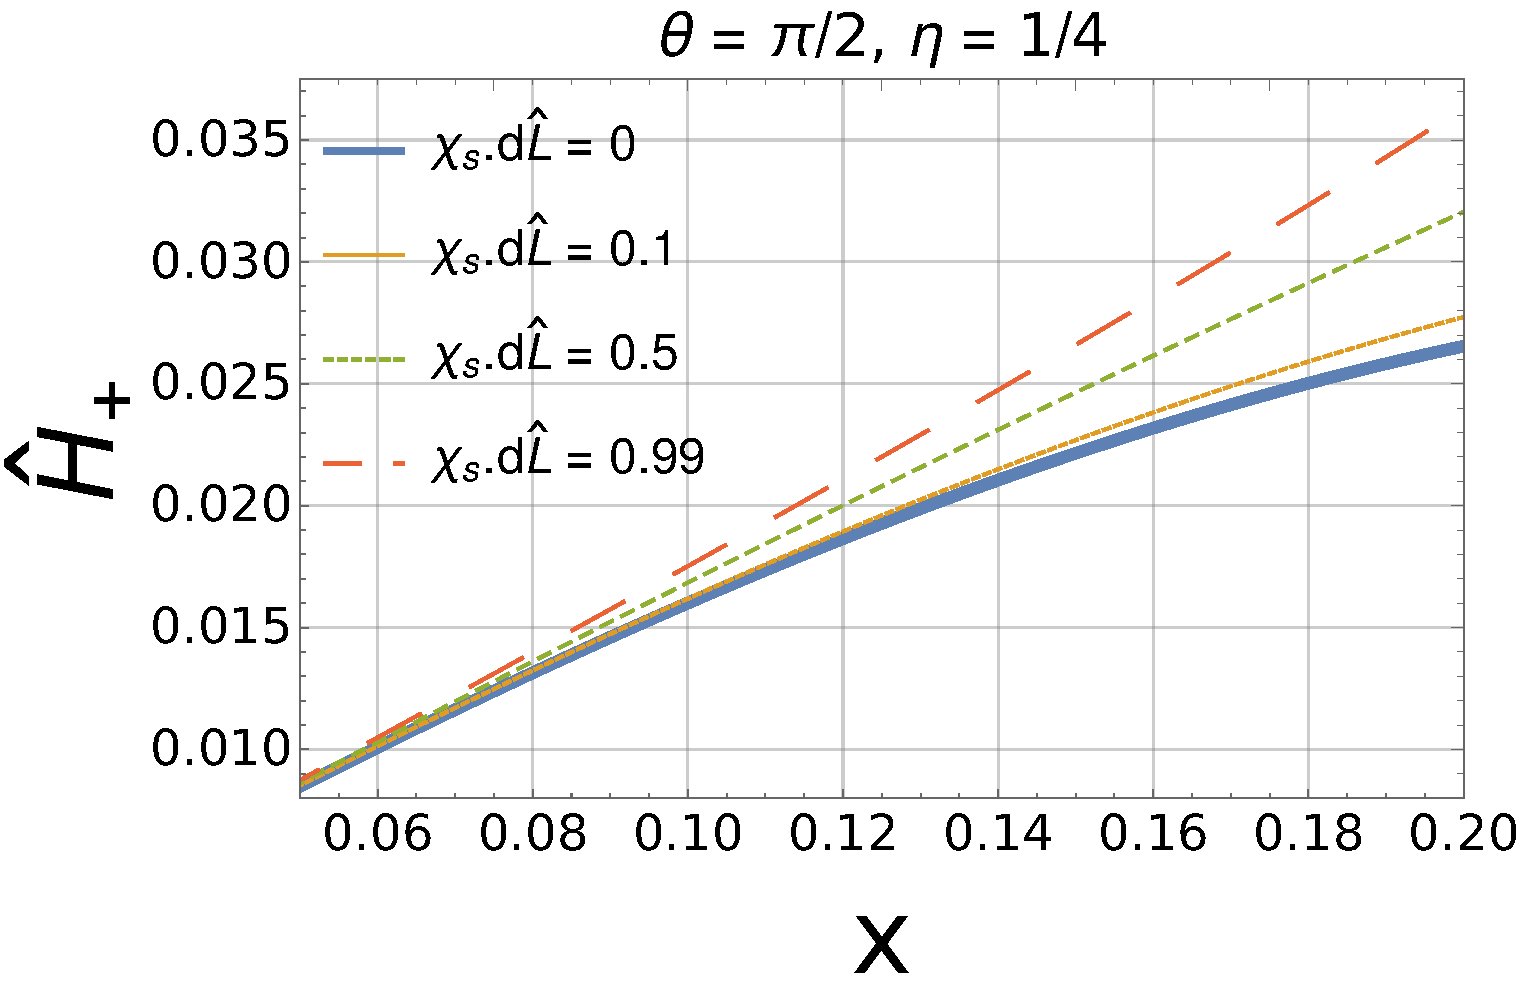
\includegraphics[width=3.5in]{../plots/PNmemorycontributionHpAlginedSpin.pdf}
	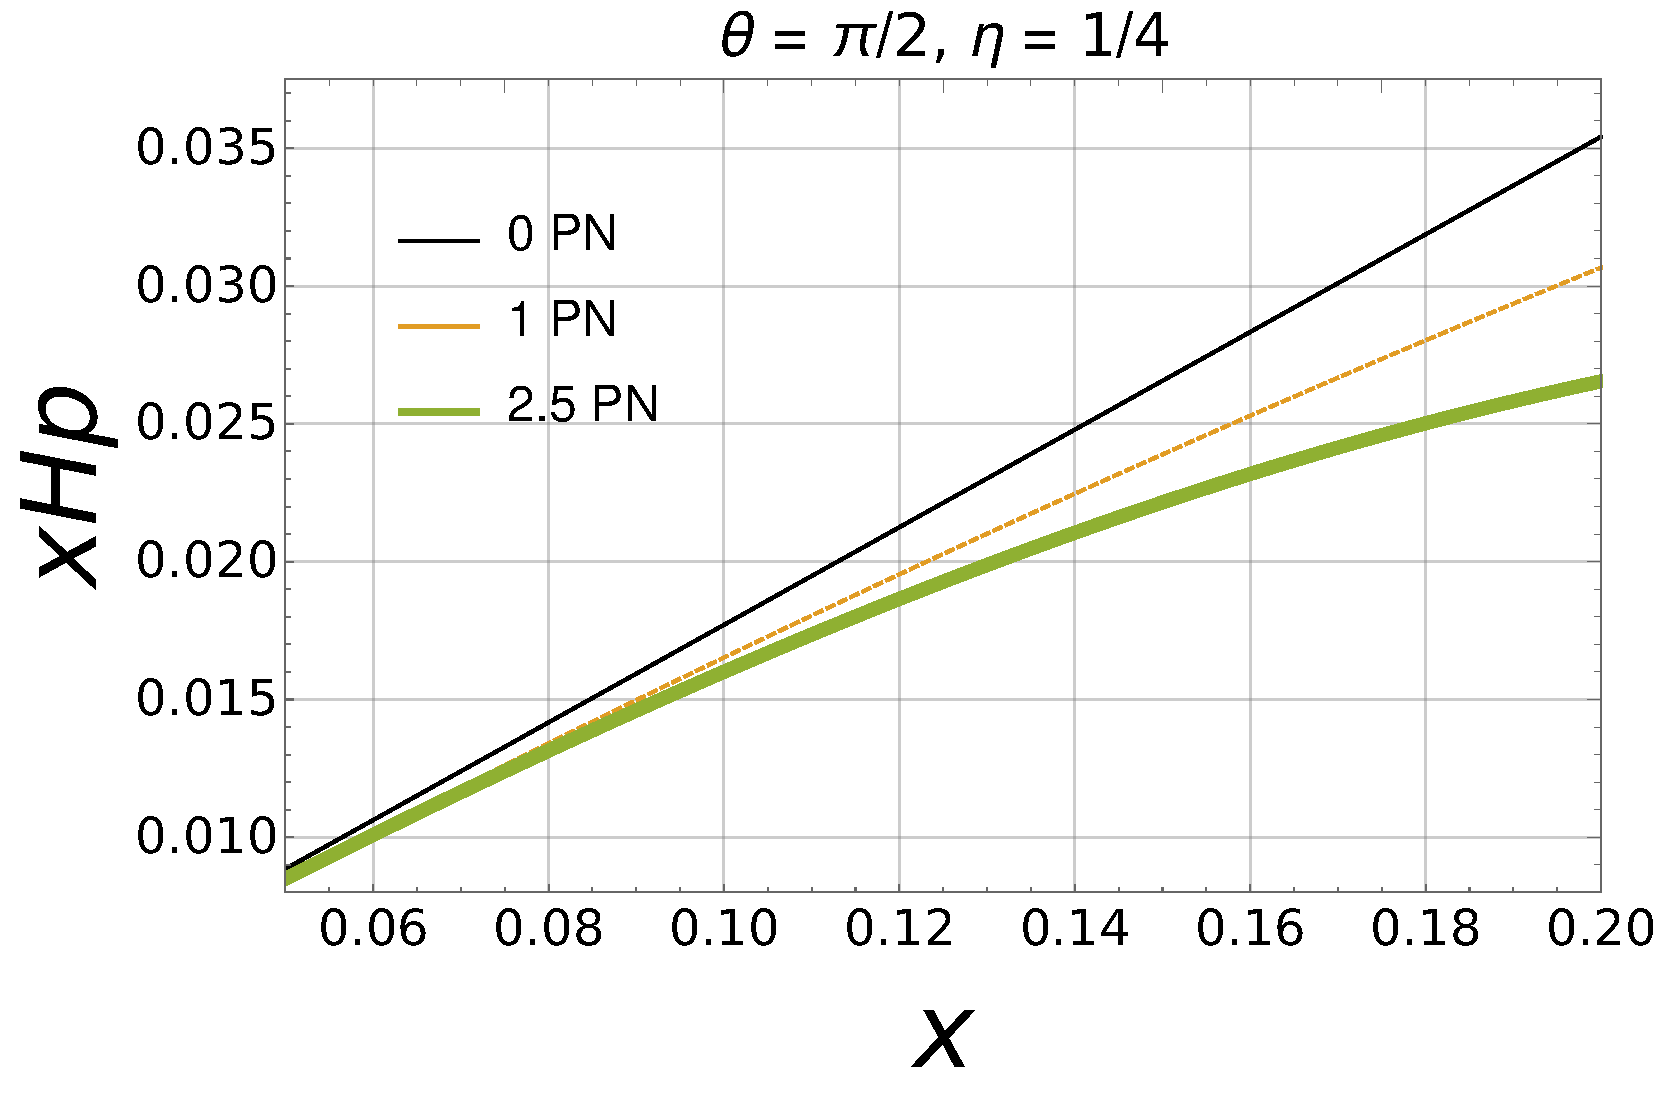
\includegraphics[width=3.5in]{../plots/PNmemoryFavata.pdf}
	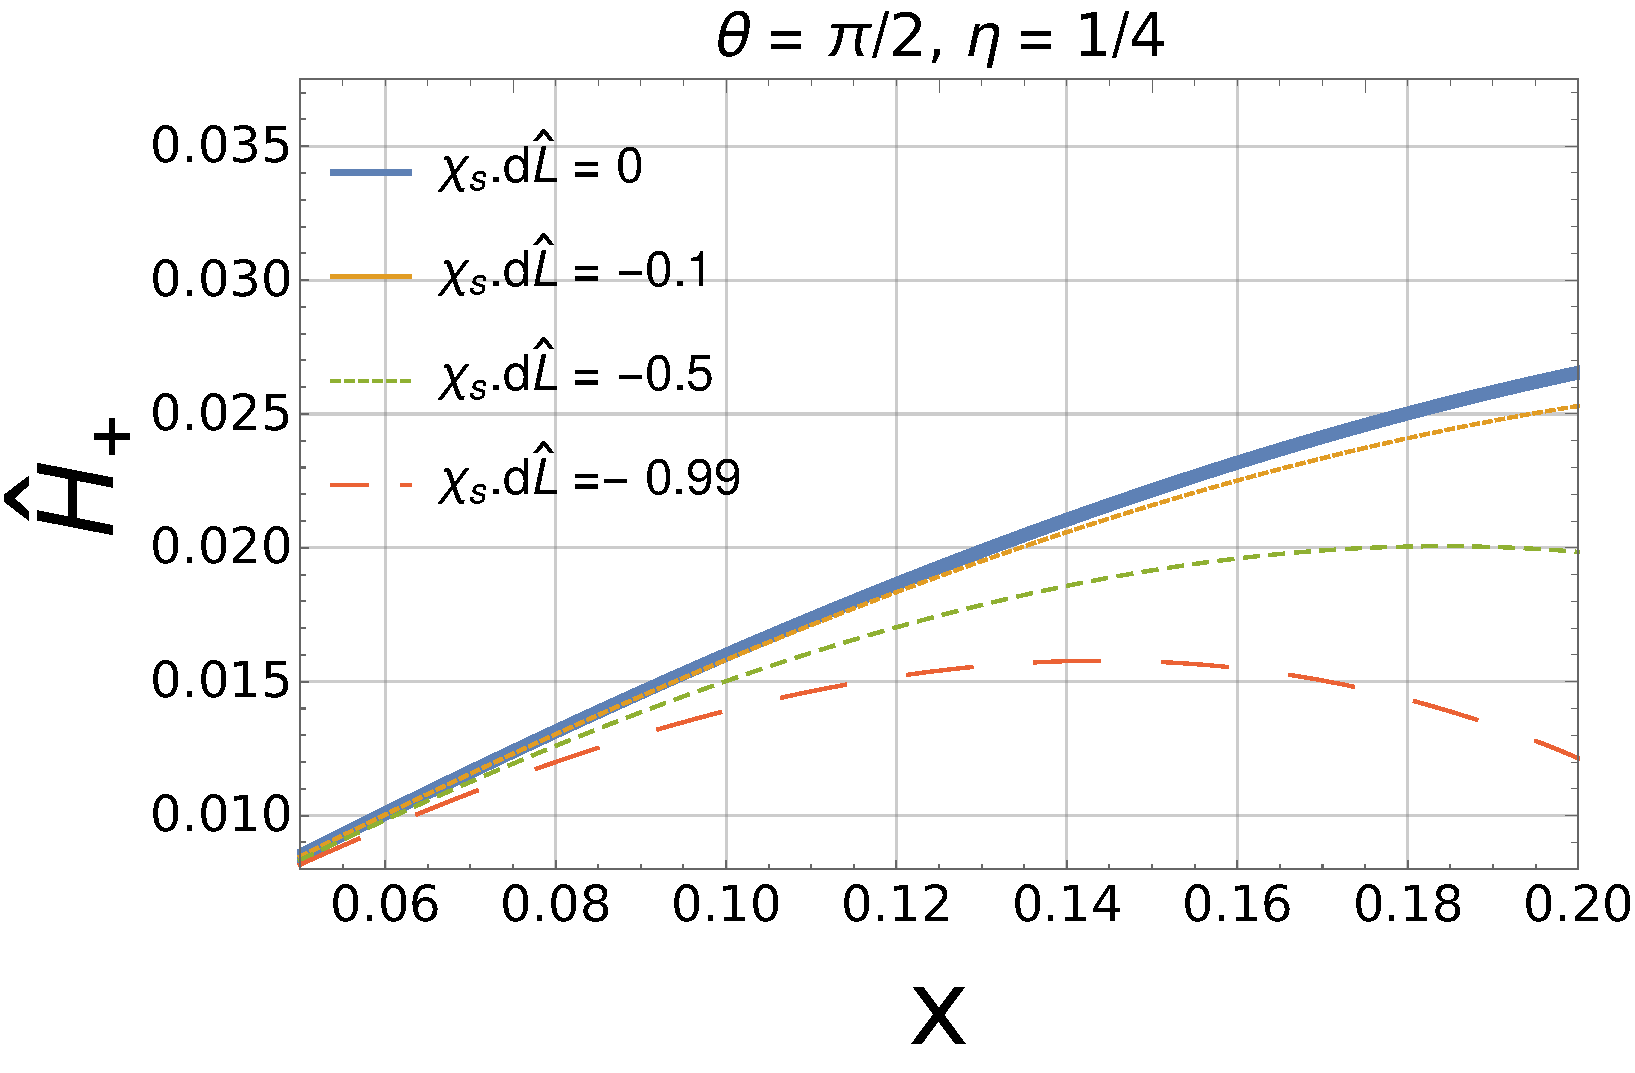
\includegraphics[width=3.5in]{../plots/PNmemorycontributionHpAntiAlginedSpin.pdf}
	\caption{Dependence of post-Newtonian (PN) corrections to the Christodoulou memory on the orbital separation. The plots above show the memory contribution to $H_+$  as a function of $x$ for different dimensionless spin parameter $\chi$ values (the polar angle to the observer at 𝛩 = 0 points along the binary orbital angular momentum) for $\eta=1/4 $ . The top left plot shows $x H_+$ as a function of parameter x which is a function of time. In plot we consider aligned spin case, where the individual spins are aligned with orbital angular momentum. It can be seen that increasing the spin magnitude tend to increase the nonlinear memory contribution. The top right figure shows the effect of including the higher PN terms to memory. this is just for comparison with Favata's results \cite{Favata2009}. The bottom figure show the effect of spin when it is anti aligned with orbital angular momentum.   
		}
	\label{fig:HpVsX}
\end{figure}
\end{widetext}

\begin{figure}
	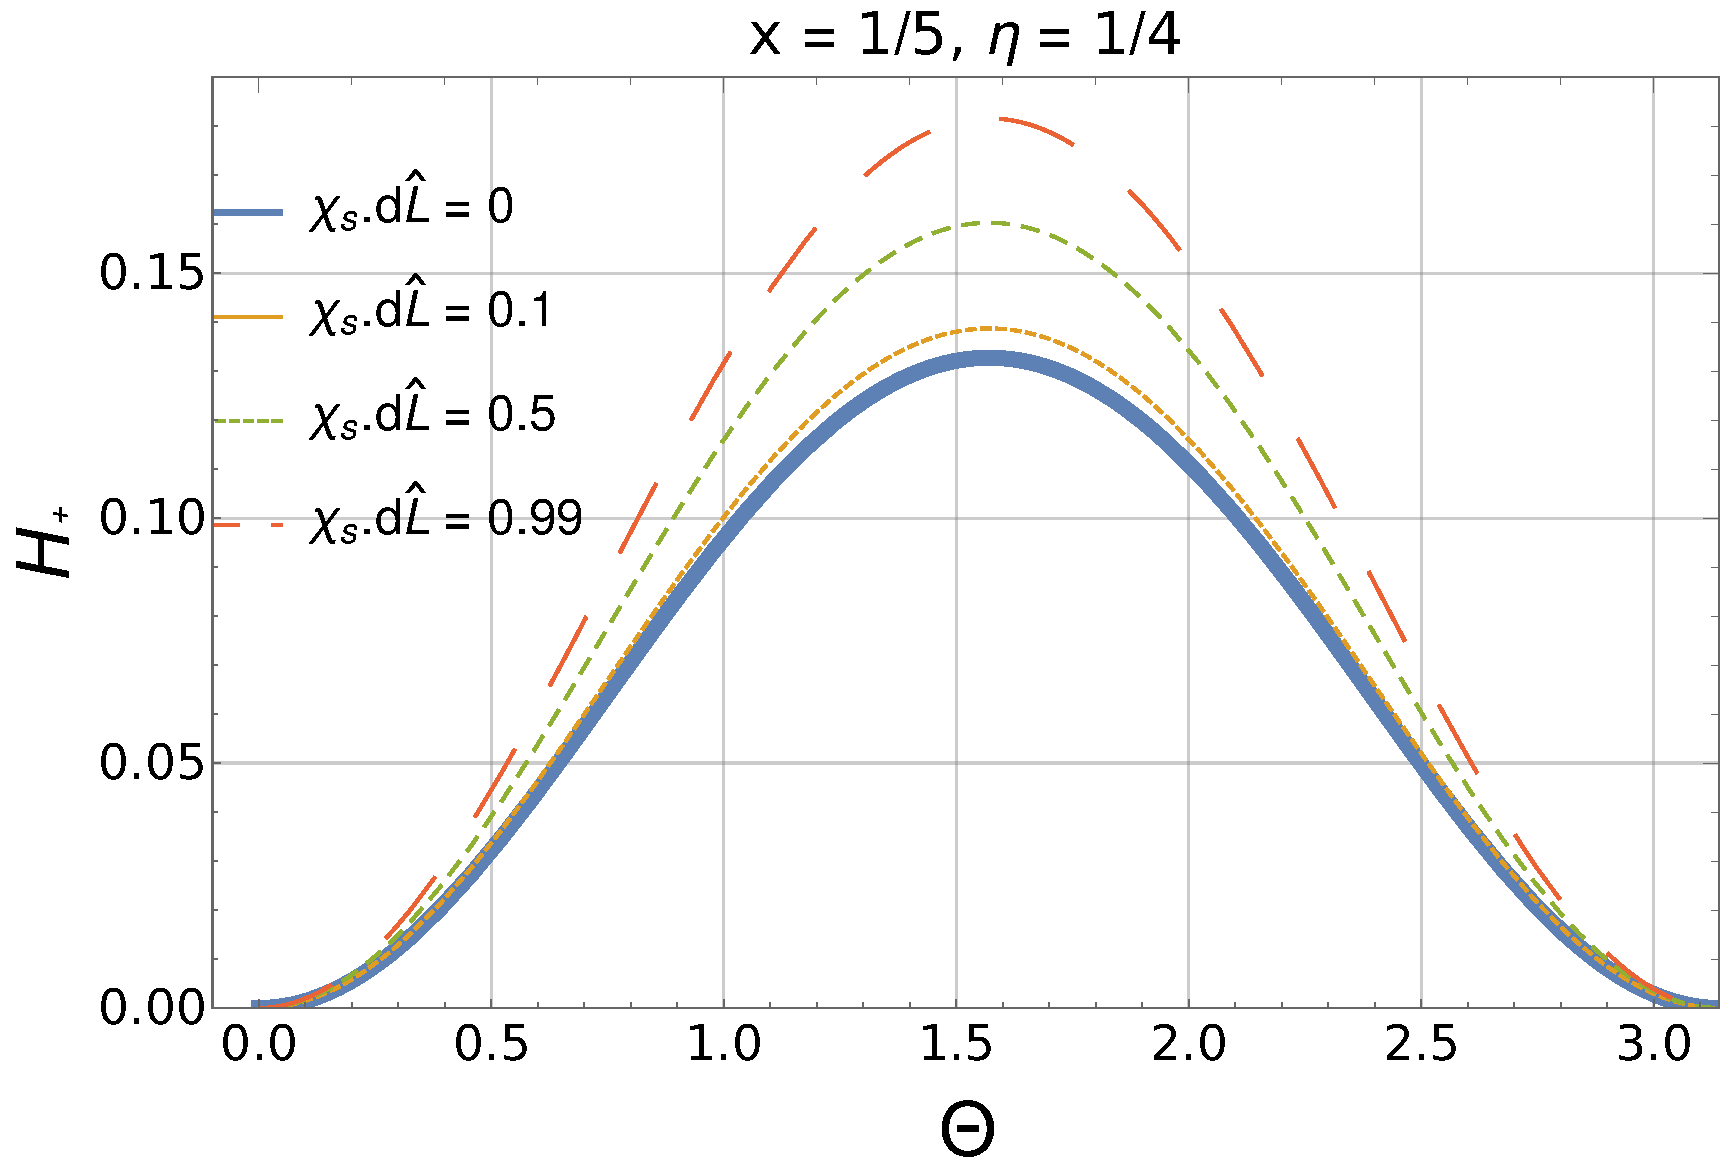
\includegraphics[width=3.5in]{../plots/PNmemorycontributionHpAlginedSpinAngular.pdf}
	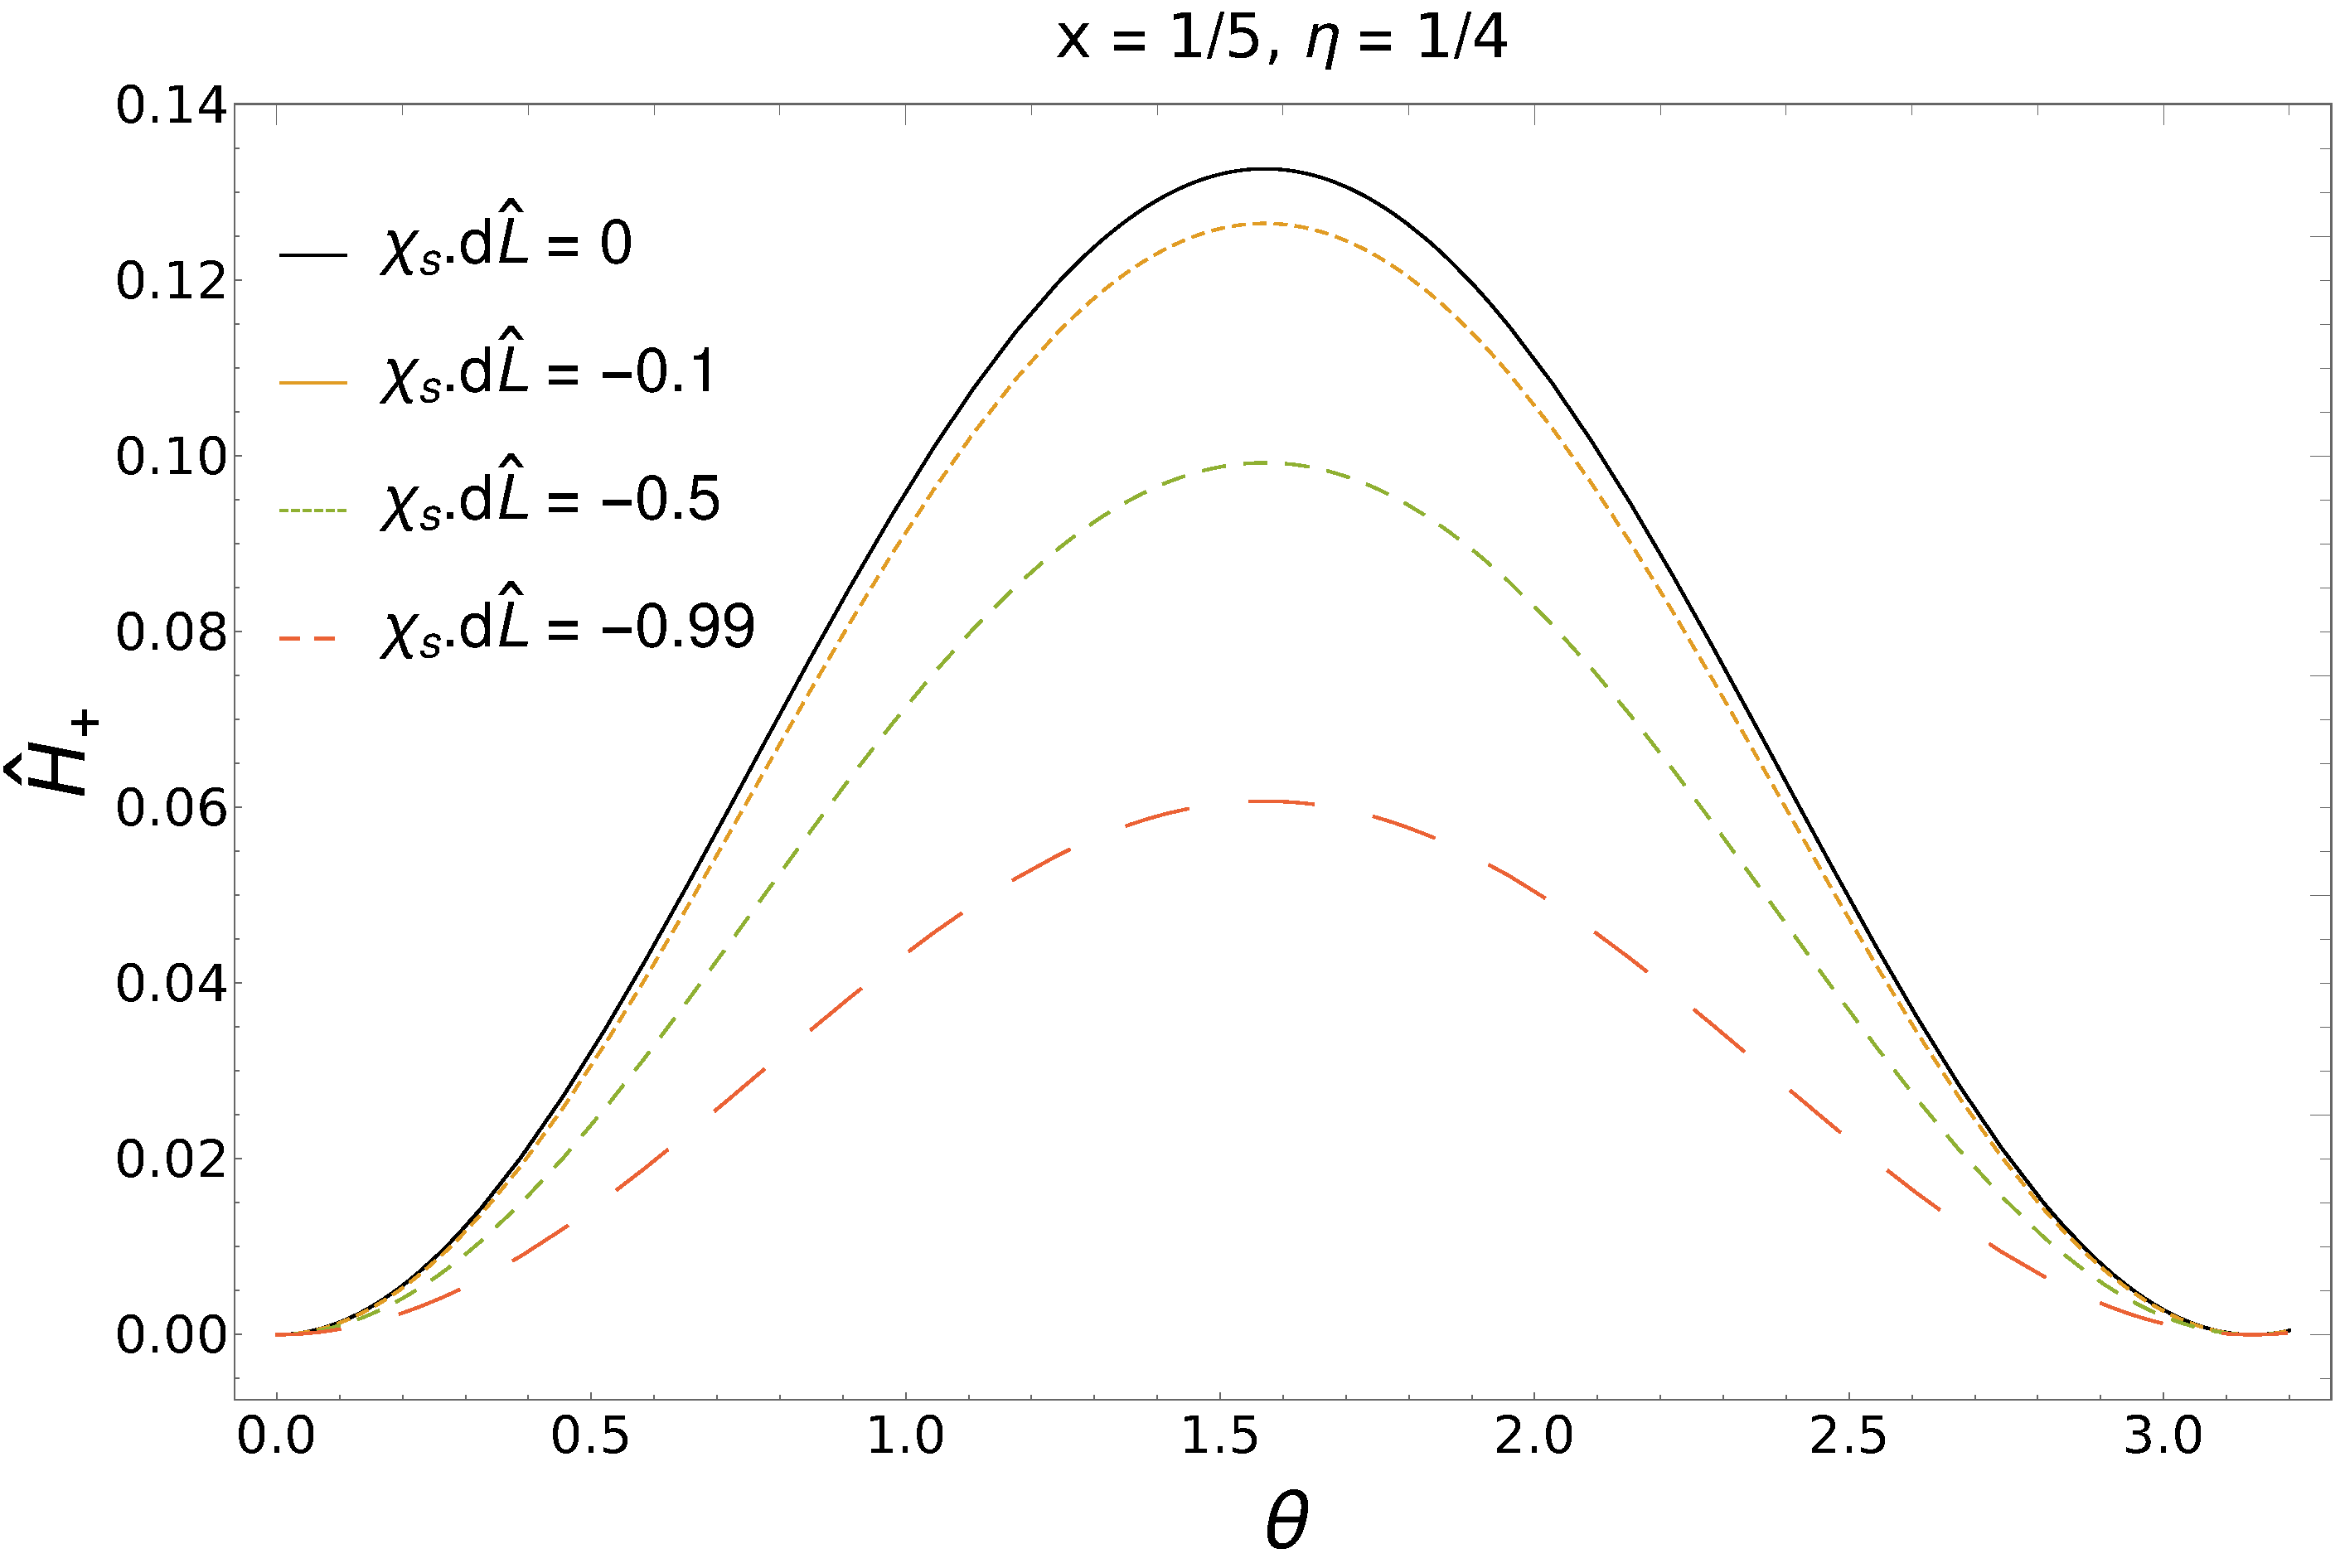
\includegraphics[width=3.5in]{../plots/PNmemorycontributionHpAntiAlginedSpinAngular.pdf}
	\caption{Dependence of post-Newtonian (PN) corrections to the Christodoulou memory on the binary inclination and orbital separation. The plots above show the memory contribution to $H_+$ for different dimensionless spin parameter $\chi$ values (the polar angle to the observer at 𝛩 = 0 points along the binary orbital angular momentum) for $x = 1/5$ and $\eta=1/4 $ . The plot to the right shows $x H_+$ as a function of parameter x. Increasing the magnitude of 𝜒 does not change the angular dependence, but does tend to increase the magnitude of the memory. 
	}
\end{figure}
\section{Memory calculation using Numerical relativity data}
Numerical relativity simulations most commonly output the Newman-Penrose curvature component $\psi_4$.The two polarization states, $h_{+}$ and $h_{\times}$ of the gravitational wave are related to the curvature, expressed in terms 	of the complex Newman-Penrose scalar $\psi_4$ by 
\begin{equation}
	\psi_4 = \ddot{h}_+ - \mathit{i}\ddot{h}_{\times}
\end{equation}\
Given the Newman-Penrose scalar $\psi_4$ for a particular mode, we have to integrate twice in time to obtain $h_{+}$ and $h_{\times}$. It has long been known that producing a strain, $h$, from the Newman-Penrose curvature component, $\psi_4$, typically results in a waveform with unphysical secular non-linear drift \cite{Berti2007}. The nonlinearity of drift indicates that this is not simply a result of two constants of integration involved in transformation. This nonlinearity is potentially caused by the fact that $\psi_4$ is typically extracted at a finite distance from the gravitating source. The strain $h$ is only related to $\psi_4$ at an infinite distance and also strictly valid in a particular gauge. As a result in numerical simulation, the finite distance calculation introduces a systematic error. In simulations \cite{Hannam2009, Reisswig2009}, which can possibly extract truly gauge-invariant waveform at future null infinity has not able able to get rid of the secular nonlinear drift.
\par It has been argued in ref. \cite{Reisswig_Pollney2011} that an important source of unphysical non-linear drift in numerical computation of gravitational wave strain lies in the transformation of the measured data to the strain $h$  which generally involves an integration in time. The output of the numerical simulation is a discretely sampled time series of finite duration, incorporating some component of unresolved frequencies due to numerical error. This can lead to an uncontrollable non-linear drift if the integration is performed in the time domain. The method described in ref \cite{Reisswig_Pollney2011} gives us a way to get rid of this unphysical behavior by eliminating the lower frequencies.    
\par The memory contribution to $h_{+}$ is given by \cite{Favata2010}

\begin{equation}\label{eq:3.2}
h_{+}^{(mem)} \approx \frac{R}{192 \, \pi}s_{\Theta}^{2}\left(17 +c_{\Theta}^{2} \right)\int_{-\infty}^{T_R}|\dot{h}_{22}|^2 dt
\end{equation}

The above equation requires a time integration of absolute value of $\dot{h}_{22}$, but this is not typically the quantity which is directly computed in numerical simulation. The output of numerical simulation is usually in the form of component of curvature tensor, or Zerilli-Moncrief-type variables defined relative to a background. 
\subsection{Evaluating Bondi News from numerical data}
The Bondi News which also the first derivative of gravitational wave strain is defined as
\begin{equation}\label{3.3}
\mathcal{N} = \int_{-\infty}^{t}dt' \psi_4
\end{equation}
The gravitational wave memory contribution to $h_{+}$ polarization can be computed from this bondi news, by integrating the absolute value of bondi news as shown in equation \ref{eq:3.2}. The memory contribution evaluated using Eq.\ref{eq:3.2} will contain contribution from numerical noise, which is unphysical and must be removed from the data. We apply the method described in the following section to remove the unphysical part of GW memory. 
\subsection{Integration of finite length signals in frequency domain}
The unphysical part of mermory essentially lies in lower frequency. A method to remove this unphysical part is given in ref \cite{Reisswig_Pollney2011}. If we remove this low frequency part from data such that the physical memory is still preserved, we can get rid of memory contribution due to numerical noise. 
Consider the Fourier transform, $\mathcal{F}$, applied to an absolutely integrable function $f(t)$,
\begin{equation}
	\tilde{f}(\omega) = \mathcal{F}[f]=\int_{-\infty}^{\infty}\e^{-\iota \omega t}f(t)dt.	
\end{equation} 
The Fourier transform of the time integral is given by
\begin{equation}
	\mathcal{F}\left[\int_{-\infty}^{t}dt' f(t')\right] |_\omega = -\iota \frac{\tilde{f}(\omega)}{\omega}
\end{equation}
The inverse fourier transform of above expression is given by
\begin{equation}\label{3.6}
	\int_{-\infty}^{t}dt'f(t')=\mathcal{F}^{-1}\left[-\mathit{i}\frac{\tilde{f}(\omega)}{\omega}\right] = -\frac{\mathit{i}}{2\pi}\int_{-\infty}^{\infty}\frac{1}{\omega}e^{\mathit{i\omega t}}\tilde{f}(\omega)d\omega
\end{equation}
In the frequency-domain, time integration becomes a simple division by the frequency. Above method is particularly susceptible to low-frequency error, under-resolved high-frequency modes can be aliased into low-frequency modes of the signal. We try to remove these unphysical frequencies by the method described below   
\subsubsection{Fixed frequency integration ($\mathit{FFI}$)}\label{FFI}
The effect of the spurious low-frequency modes caused by spectral leakage or aliasing effects, can be significantly suppressed by use of signal filter. The time integral can be performed in frequency domain as shown in equation \ref{3.6}. The low frequencies which cause the unphysical nonlinear drift can be removed by choosing a cutoff frequency while taking a Fourier transform.   

\[\tilde{F} =
\begin{cases}
-\mathit{i} \frac{\tilde{f}(\omega)}{\omega_0} & \text{ $\omega\leq\omega_0$} \\
-\mathit{i} \frac{\tilde{f}(\omega)}{\omega} & \text{ $\omega>\omega_0$} 
\end{cases}\]

We use this method to integrate $\psi$ to obtain Bondi News as shown in equation \ref{3.3}.

\subsection{Memory calculation from SXS Rumerical Relativity data}
The publicly available SXS catalog provides data for Newman-Penrose scalar component $\psi_4$, decomposed into spin weighted spherical harmonics, extrapolated to infinite radius. We used this data and  performed a frequency domain time integration as described in equation \ref{3.6}, while removing the unphysical frequency by choosing a lower cutoff as show in section \ref{FFI}. The cutoff frequency is chosen as $\omega_0/10$ where $\omega_0$ is the minimum instantaneous GW angular frequency. We first begin by separating the complex Newman-Perose scalar $\psi_4$ data into phase and amplitude part. We compute instantaneous GW angular frequency from this by taking the first time derivative of phase corresponding to $\psi_4$. The instantaneous GW frequency often looks noisy at the beginning of the simulations due to numerical issues. We remove this noise data by choosing a lower and upper cutoff time. Once we find the upper and lower cutoff time, we can apply a frequency domain time integration for $\psi_4$ by choosing a cutoff frequency. After filtering the noise creating frequency we can use equation \ref{eq:3.2} to compute the memory contribution to "plus" polarization of GW signal. The SXS catalog gives data for different parameter values like mass ratio, dimensionless spin parameter etc. The Christodoulou memory computed from Numerical Relativity data starts from zeros using equation \ref{eq:3.2} due to finite simulation time. Chrostodoulou memory is hereditary, hence it's entire past should be included. This can be done by combining the PN expression during early inspiral and numerical relativity results for merger part. The method used to connect the memory accumulated during entire life time of BBH coalesce is described in the next section. 
\subsection{Compleate Christodoulou memory during BBH coalescence} 
The PN waveform for Christodoulou are given as a function of parameter $x$ which is related to time by equation \ref{eq:2.14}. This equation can be integrated to obtain a relation between time $t$ and parameter $x$. The Christodoulou memory reaches it's peak value at the merger. We choose the values of integration constants such that the peak in $h_+^{(mem)}$ is reached at time $t=0$. We use our PN results for computing the memory during early inspiral and attach them to NR results near the late inspiral. We compare this memory for different mass ratio and different values of dimensionless spin parameter. Figure \ref{fig:differentmassratio} show the Christodoulou memory for different mass ratios, which shows that the Christodoulou tends to decrease with higher mass ration. The effect of dimensionless spin is shown in figure \ref{fig:differntchivalues}. It can be seen that the spin magnitude has significant effect on nonlinear memory, higher spin magnitude, in case of spin aligned with orbital angular momentum tends to increase the memory contribution. When the spins are anti aligned with orbital angular momentum, it tend to decrease the Christodoulou memory. These results show that it is important to consider the spin contribution when studying the Christodoulou memory in gravitational wave signals. 

%%%%%%%%%%%%%%%%%%%%%%%%%%%%%%%%%%%%%%%%%%%%%%%%%%%%%%%%

\begin{figure}
 	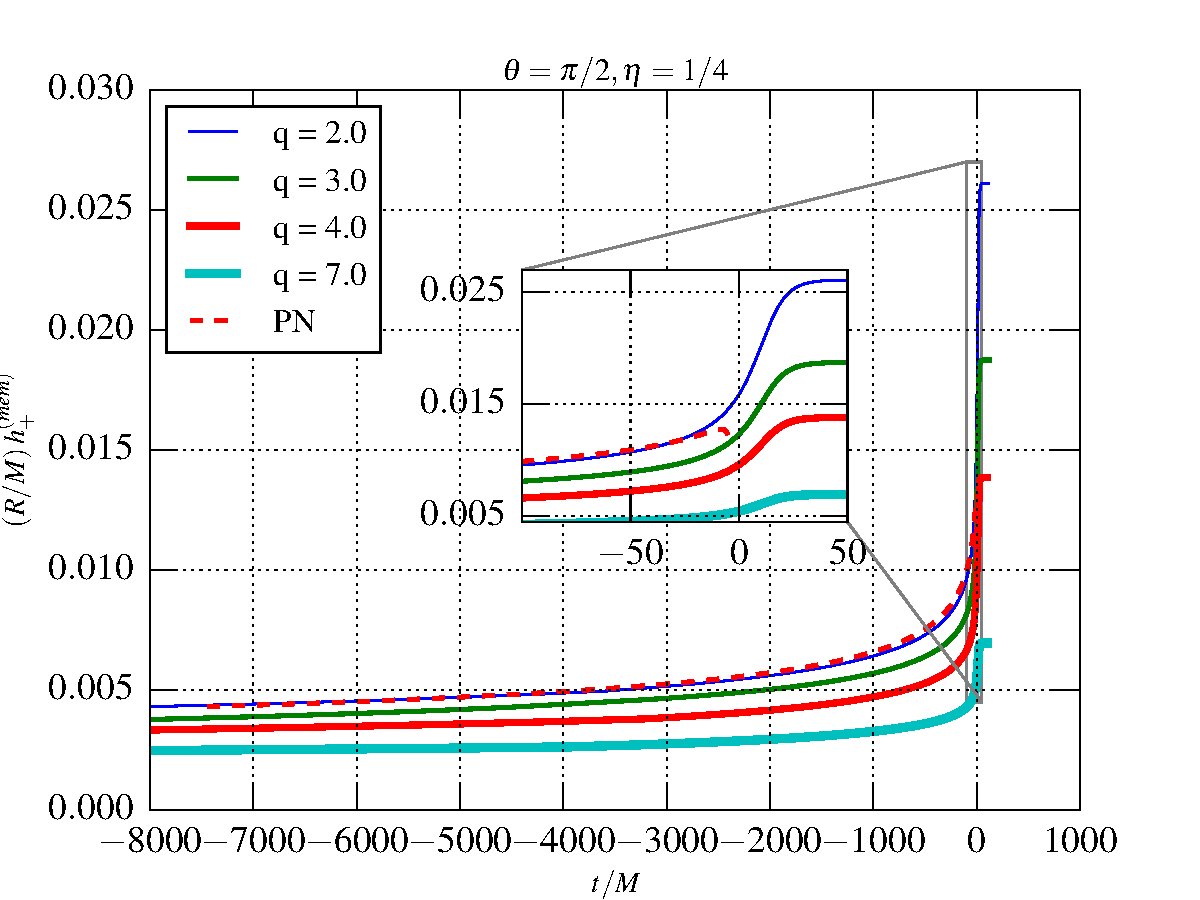
\includegraphics[width=4.0in]{../plots/MemoryPlot_nonSpining/q7.pdf}
 	\caption{The figure above shows Christodoulou memory as a function of time during BBH coalesce. This figure shows a comparison for different mass ratios. It can be seen that higher mass ration tends to decrease the Chistodoulou memory. The early inspiral part is computed using post-Newtonian expression and the later part during BBH merger is computer using Numerical Relativity data. The red dashed line shows result from PN expression}
 	\label{fig:differentmassratio}
\end{figure}
\begin{figure}
	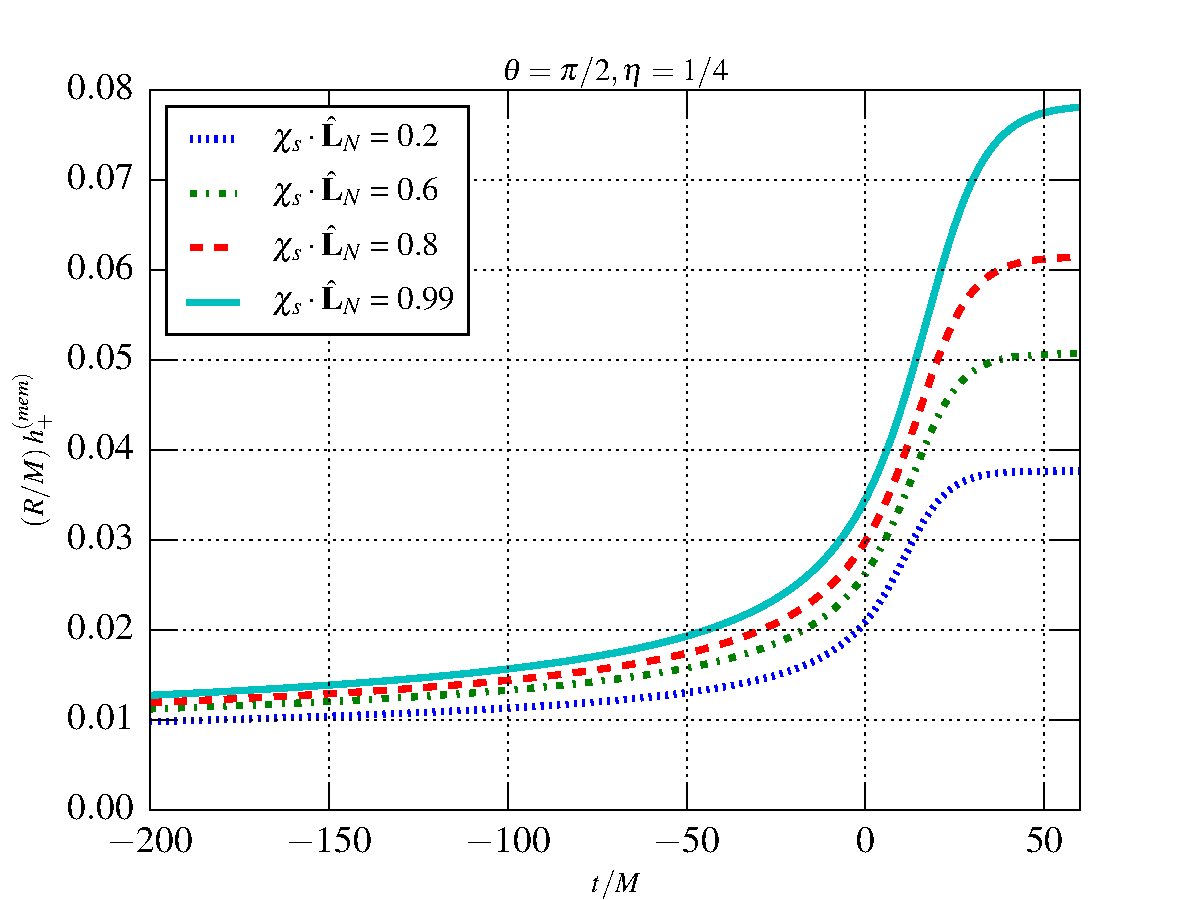
\includegraphics[width=4.0in]{../plots/MemoryPlot_AlignedSpinSXSdata/0p99.pdf}
	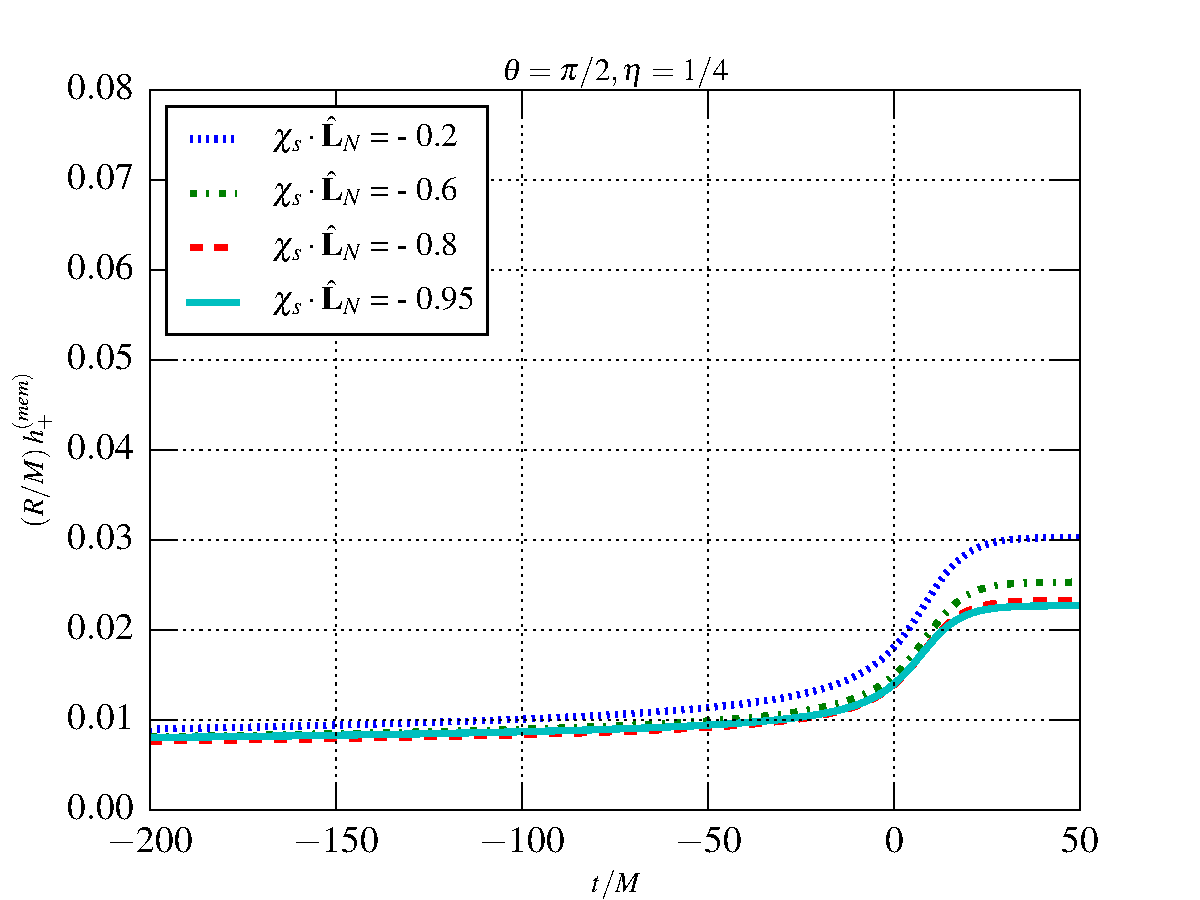
\includegraphics[width=4.0in]{../plots/MemoryPlot_AntialignedSpinSXSdata/m0p94.pdf}
	\caption{The figure above shows Christodoulou memory as a function of time during BBH coalesce. The top figure shows a comparison for different values of dimensionless spin parameter $\chi$. These results are for BBH system with equal spin magnitude for individual black hole and spins aligned with orbital angular momentum. It can be seen that higher spin magnitude tend to increase the Christodoulou memory. The bottom figure shows the anti aligned case.  }
	\label{fig:differntchivalues}
\end{figure}

\subsection{CONCLUSIONS}
Observation of Christodoulou memory would be an important test of general relativity in strong field regime. Effort to detect this memory effect in low frequency band from super massive black holes have been undertaken by pulsar timing array experiments \cite{Pshirkov2010}. In these experiment the spin effect have been neglected for modeling the signal. It is highly likely that super massive black holes have significant spin due to accretion of matter from surrounding. We have shown in this paper that spin contribution can significantly change the Christodoulou memory. Hence it is important to consider the spin effect while modeling the signals.

\section{Acknowledgments}
We thank the West Virginia Univerisity. This work was support by ... 

\newpage
\appendix 
\begin{widetext}

\section{Angular Integral Of The Triple Product Of Spin-Weighted Spherical Harmonics}\label{Appendix A}
The following integral appears in the evaluation of nonlinear memory contribution to the radiative mass-multipole moments $U_{lm}$. Equation 2.4 can be rewritten as
\begin{equation}
	d^{\,l_j}_{m_js_j}(\Theta)=\sum_{k_j=k_i(j)}^{k_f(j)}g_j(k_j)\left(\sin\frac{\Theta}{2}\right)^{p_j}\left(\cos\frac{\Theta}{2}\right)^{2l_j-p_j}
\end{equation}
where
\begin{equation}
	g_j(k_j)=\frac{(-1)^k_j[(l_j + m_j)!(l_j-m_j)!(l_j+s_j)!(l_j-s_j)!]^{1/2}}{k_j!(l_j+m_j-k_j)!(l_j-s_j-k_j)!(s_j-m_j+k_j)!},
\end{equation}
$p_j=2k_j+s_j-m_j$, $k_i=\max(0, m-s)$ and $k_f=\min(l+m, l-s)$. The index $j=1,2,3$ serves only the three harmonics. The required integral can be written as:

\begin{align}
	G^{s_1 s_2 s_3}_{l_1 l_2 l_3 m_1 m_2 m_3}&\equiv\int\, _{-s1}Y^{l_1m_1}(\Theta, \Phi)_{-s2}Y^{l_2m_2}(\Theta, \Phi)_{-s3}Y^{l_3m_3}(\Theta, \Phi)d\Omega \nonumber \\
	&=(-1)^{s_1+s_2+s_3}\frac{[(2l_1+1)(2l_2+1)(2l_3+1)]^{1/2}}{(4\pi)^{3/2}}\int_{0}^{2\pi}e^{\mathit{i}(m_1+m_2+m_3)\Phi}d\Phi\int_{0}^{\pi}d^{l_1}_{m_1s_1}d^{l_2}_{m_2s_2}d^{l_3}_{m_3s_3}\sin(\Theta)d\Theta
\end{align}
The $\Phi$ integral is 
\begin{equation}
	\int_{0}^{2\pi}e^{\mathit{i}(m_1+m_2+m_3)\Phi}d\Phi = 2\pi\delta^{-m_1}_{m_2+m_3}
\end{equation}
The $\Phi$ integral can be written as 
\begin{equation}
	\int_{0}^{\pi}d^{l_1}_{m_1s_1}d^{l_2}_{m_2s_2}d^{l_3}_{m_3s_3}\sin\Theta d\Theta = 2\sum_{k_1k_2k_3}g_1(k_1)g_2(k_2)g_3(k_3)\int_{0}^{\pi}\left(\sin\frac{\Theta}{2}\right)^{2a-1}\left(\cos\frac{\Theta}{2}\right)^{2b-1}d\Theta
\end{equation}
where $a=1+(p_1+p_2+p_3)/2$ and $b=1+l_1+l_2+l_3-(p_1+p_2+p_3)/2$. The $\Phi$ integral is expression in terms of the Beta or Gamma function and can be found in standard tables.
\begin{equation}
	\int_{0}^{\pi}\left(\sin\frac{\Theta}{2}\right)^{2a-1}\left(\cos\frac{\Theta}{2}\right)^{2b-1}d\Theta=\frac{\Gamma(a)\Gamma(b)}{\Gamma(a+b)}=B(a,b)
\end{equation}

\section{Calculation Of The $\dot{h}_{lm}$ Modes}\label{Appendix B}
The $h_{lm}$ modes are written as 
\begin{equation}\label{eq:B1}
	h_{lm}=8\sqrt{\frac{\pi}{5}}\frac{\eta\,M}{R}x\hat{H}_{lm}(x)e^{\mathit{i}m\psi}
\end{equation}
where the $\hat{H}_{lm}$ are obtained by taking the non-precessing limit of expressions for precessing binaries given in Ref.\cite{Arun2009} . In this paper we are interested in nonprecessing case, so we rewrite the expressions such that spin are aligned with the total orbital angular momentum. The phase variable $\psi$ is related to the orbital phase $\phi$ via
\begin{equation}
	\psi=\varphi - 3x^{3/2}\left[1-\frac{\eta}{2}x\right]\ln\left(\frac{x}{x_0}\right)
\end{equation}
where $\ln x_0 = \frac{11}{18} - \frac{2}{3}\gamma_E -\frac{4}{3}\ln2 + \frac{2}{3}\ln\left(\frac{M}{r_0}\right)$ is related to the arbitrary constant $r_0$ appearing in the coordinate transformation of Eq. (2.20) or ref\cite{Favata2009}. The orbital phase can be expressed a function of x for nonprecessing binaries, to 3.5PN order.This expression is given in Eq(3.4) of Ref. \cite{Ajith_2011}
\begin{align}
\varphi(x)& = -\frac{1}{32\,\eta\,x^{5/2}}\left\{1+x\left[\frac{55\eta}{12}+\frac{3715}{1008}\right]+x^{3/2}\left[\frac{565}{24}\left(\left(1-\frac{76\eta}{133}\right)\chisdL + \delta\chiadL\right)-10\pi\right]\right.\nonumber\\
&\quad + x^2\left[\left(\chiadL\right)^2\left(150\eta-\frac{3595}{96}\right)-\frac{3595\chiadL\chisdL\delta}{48} + \chiaSqr\left(\frac{1165}{96}- 50\eta\right) + \frac{1165\chisDchia\delta}{\delta}\right]\nonumber\\
&\qquad + \left.\left(\chisdL\right)^2\left(-\frac{5\eta}{24} - \frac{3595}{96}\right) + \chisSqr\left(\frac{35\eta}{24}+\frac{1165}{96}\right) + \frac{3085\eta^2}{144} + \frac{27145\eta}{1008} + \frac{15293365}{10160664}\right]\nonumber\\
&\quad +  \frac{x^{5/2}}{2}\left[\left(\chiadL\left(-\frac{35\delta\eta}{2} - \frac{732985\delta}{2016}\right) + \chisdL\left(\frac{85\eta^2}{2} + \frac{6065\eta}{18} - \frac{732985}{2016}\right) -\frac{65\pi\eta}{8} + \frac{38645\pi}{672}\right)\ln(x)\right]\nonumber\\
&\quad x^3\left[-\frac{127825\eta^3}{5184} + \frac{76055\eta^2}{6912} + \frac{2255\pi^2\eta}{48} - \frac{15737765635\eta}{12192768} - \frac{1712\gamma_E}{21} -\frac{160\pi^2}{3} + \frac{12348611916451}{18776862720} - \frac{1712\ln(16x)}{42}\right]\nonumber\\
&\quad \left.x^{7/2}\left[-\frac{74045\pi\eta^2}{6048} + \frac{378515\pi\eta}{12096} + \frac{77096675\pi}{2032128}\right]\right\}
\end{align} 
where $\varphi_0$ is a certain reference phase. The first time derivative of modes can be obtained by using equation \ref{eq:B1} and substituting the expression for $\dot{x}$ as a function of $x$ using Eq. \ref{eq:C3}. We use the expression for time derivative as show in equation below
\begin{equation}
	\dot{h}_{lm} = 8\sqrt{\frac{\pi}{5}}\frac{\eta\,M}{R}\dot{x}e^{-\mathit{i}m\psi}\left(\tilde{H}_{lm}' - \mathit{i}m\psi'\tilde{H}_{lm} \right)
\end{equation}
where the prime denotes the derivative with respect to $x$.

\section{Complete 3.5 PN expressions for Energy and Flux}\label{Appendix:C}

\begin{align}\label{Appendix:C1}
E&=-\frac{\eta \, M \, x}{2}\left\{1 + x \left[-\frac{3}{4}-\frac{\eta}{12}\right] + x^{3/2}\left[\left(\frac{8}{3} - \frac{4 \, \eta}{3}\right)\chisdL + \frac{8}{3}\delta\chiadL\right]\right. \nonumber \\
& \quad \left. x^2\left[-\frac{27}{8} + \frac{19 \, \eta}{8}-\frac{\eta^2}{24} + \eta^2 \left\{\left(\chisSqr-\chiaSqr\right) -3\left[\left(\chisdL\right)^2 - \left(\chiadL\right)^2\right]\right\}\right.\right. \nonumber \\
& \qquad \left(\frac{1}{2}-\eta\right)\left\{\chisSqr+\chiaSqr-3\left[\left(\chisdL\right)^2+\left(\chiadL\right)^2\right]\right\}+\delta\left\{\chisDchia-3\left[\left(\chisdL\chisdL\right)\right]\right\} \nonumber\\
& \quad \left.\left.x^{5/2}\left[\left(8-\frac{121\,\eta}{9} +  \frac{2\,\eta^2}{9}\right)\chisdL + \left(8-\frac{31\,\eta}{9}\right)\delta\chiadL\right] + x^3\left[-\frac{675}{64}+\left(\frac{34445}{576}-\frac{205\,\pi^2}{96}\right)\eta-\frac{155\,\eta^2}{96}-\frac{35\,\eta^3}{5184}\right]
\right]
\right\}\nonumber\\
\\
\label{Appendix:C2}
\mathcal{L}&=\frac{32}{5}\eta^2x^5\left\{1 + x\left[-\frac{1247}{336}-\frac{35\,\eta}{12}\right] + x^{3/2}\left[4\pi-\left\{\left(\frac{11}{4}-3\eta\right)\chisdL +\frac{11}{4}\delta\chiadL\right\}\right]\right.\nonumber\\
&\quad  x^2\left[-\frac{44711}{9072}+\frac{9271\eta}{504}+\frac{65\, \eta^2}{18} + \left(\frac{287}{96} +\frac{\eta}{24}\right)\left(\chisdL\right)^2-\left(\frac{89}{96}+\frac{7\,\eta}{24}\right)\chisSqr\right.\nonumber\\
&\qquad\left. + \left(\frac{287}{96}-12\eta\right)\left(\chiadL\right)^2 + \left(-\frac{89}{96}+4\eta\right)\chiaSqr + \frac{287}{48}\delta\left(\chisdL\right)\left(\chiadL\right) -\frac{89}{48}\delta\left(\chisDchia\right)\right]\nonumber\\
&\quad\left.x^{5/2}\left[\left(-\frac{8191}{672}-\frac{583\,\eta}{24}\right)\pi+\left\{\left(-\frac{59}{16}+\frac{227\, \eta}{9}-\frac{157\, \eta^2}{9}\right)\chisdL + \left(-\frac{59}{16} + \frac{701\,\eta}{36}\delta\chiadL\right)\right\}\right.\right]\nonumber\\&\quad \left.x^3\left[\frac{6643739519}{69854400}+\frac{16\,\pi^2}{3}-\frac{1712\,\gamma_E}{105}-\frac{856}{105}\log(16x)+\left(-\frac{134543}{7776}+\frac{41\,\pi^2}{48}\right)\eta -\frac{94403\,\eta^2}{3024}-\frac{775\,\eta^3}{324}
\right]\right\}\nonumber\\
\\
\label{eq:C3}
\frac{dx}{dt}&=\frac{64\, x^5  \, \eta}{5}\left\{1 + x \left[-\frac{743}{336}-\frac{11 \eta }{4} \right] 
+ x^{3/2} \left[4 \pi-\frac{113}{12}\delta \, \chiadL- \left(-\frac{113}{19} + \frac{19 \, \eta}{3}  \right)\chisdL \right] \right. \nonumber \\
&\quad + x^2 \left[ \frac{34103}{18144} + \frac{13661 \, \eta}{2016} + \frac{59 \, \eta^2}{18} + \left( \frac{719}{96}- 30 \eta\right)(\chiadL)^2 +\chiaSqr \left(-\frac{233}{96}+10 \eta \right) \right. \nonumber\\
&\qquad+\frac{719 \chiadL \, \chisdL \delta}{48}-\frac{233 \chisDchia \delta}{48} \left. + \, (\chisdL)^2 \left(-\frac{\eta }{24}-\frac{719}{96}\right)+\chisSqr \left(\frac{7 \eta
}{24}+\frac{233}{96}\right) \right] \nonumber \\ 
&\quad + x^{5/2} \left[-\frac{4159 \, \pi}{672}-\frac{189 \, \pi \, \eta}{8} + \chiadL \delta  \left(-\frac{31319}{1008} + \frac{1159 \, \eta}{24}\right)+\chisdL \left(-\frac{31319}{1008} + \frac{22975 \, \eta}{252} -\frac{79 \, \eta^2}{3}\right) \right]  \nonumber\\ 
&\quad \left. + x^3 \left[\frac{16447322263}{139708800} + \frac{16 \, \pi^2}{3} -\frac{1712 \, \gamma_{E}}{105} -\frac{56198689 \, \eta}{217728} + \frac{451 \, \pi^2 \, \eta}{48} + \frac{541 \, \eta^2}{896} -\frac{5605 \, \eta^{3}}{2592} -\frac{80 \,\pi \delta\chiadL }{3} \right.\right. \nonumber \\
&\qquad \left.\left. + \left(\frac{575}{448} + \frac{565 \, \delta^2}{9}-\frac{65815 \, \eta}{4032} + \frac{89 \, \eta^2}{2}\right)(\chiadL)^2 + \left(-\frac{145}{448}+\frac{21985 \,\eta}{4032} -\frac{89 \, \eta^2}{6}\right)\chiaSqr + \right(-\frac{80 \, \pi}{3} + \frac{40 \, \pi \, \eta}{3} \right. \nonumber \\
&\qquad  \left.+\delta\left(\frac{258295}{2016} -\frac{9203 \, \eta}{96}\right)\chiadL\left)\chisdL + \left(\frac{258295}{4032} -\frac{48773 \, \eta}{576} + \frac{3041 \, \eta^2}{144}\right)(\chisdL)^2 + \delta\left(-\frac{145}{224} + \frac{2143 \, \eta}{288}\right)\chisDchia \right.\right.\nonumber \\ 
&\qquad\left.\left.+\left(-\frac{145}{448} + \frac{1891 \, \eta}{576} -\frac{7 \, \eta^2}{144}\right)\chisSqr - \frac{3424 \, \log[2]}{105} - \frac{1712 \log[x]}{210}\right]\right\}
\end{align}
\end{widetext}


\section*{References}

\bibliographystyle{apsrev4-1}
\bibliography{references}

\end{document}
